\documentclass[letterpaper,11pt]{article}

\usepackage[margin=1in]{geometry}
\usepackage[tight,nice]{units}
\usepackage{graphicx,color,float,url,amsmath,parskip,multicol}
%\usepackage[super]{cite}
\usepackage{subfigure}
\usepackage{listings}
\usepackage{sectsty}
\usepackage{appendix}
\usepackage{amssymb}
\usepackage{url}
\sectionfont{\normalsize}
\subsectionfont{\normalsize}
\title{\normalsize}
\usepackage{setspace}
\usepackage{natbib}
\usepackage[nottoc,numbib]{tocbibind}
\usepackage{fancyhdr}
\usepackage[outercaption]{sidecap}
\usepackage{eqnarray}
\usepackage{mathrsfs, amsmath, amsfonts, xspace}
\usepackage[pagewise, mathlines]{lineno}

\usepackage{hyperref}
\hypersetup{colorlinks=true,linkcolor=blue,citecolor=blue}

%% =============================================================================
%% My eqs
%% =============================================================================
\renewcommand{\bibname}{REFERENCES}
\newcommand{\SimPEG}{\textsc{SimPEG}\xspace}
\renewcommand{\div}{\nabla\cdot}
\newcommand{\grad}{\vec \nabla}
\newcommand{\curl}{{\vec \nabla}\times}
\newcommand {\J}{{\vec J}}
\renewcommand{\H}{{\vec H}}
\newcommand {\E}{{\vec E}}
\newcommand{\siginf}{\sigma_\infty}
\newcommand{\dsig}{\triangle\sigma}
\newcommand{\dcurl}{{\mathbf C}}
\newcommand{\dgrad}{{\mathbf G}}
\newcommand{\Acf}{{\mathbf A_c^f}}
\newcommand{\Ace}{{\mathbf A_c^e}}
\renewcommand{\S}{{\mathbf \Sigma}}
\newcommand{\St}{{\mathbf \Sigma_\tau}}
\newcommand{\T}{{\mathbf T}}
\newcommand{\Tt}{{\mathbf T_\tau}}
\newcommand{\diag}{\mathbf{diag}}
\newcommand{\M}{{\mathbf M}}
\newcommand{\MfMui}{{\M^f_{\mu^{-1}}}}
\newcommand{\MfMuoi}{{\M^f_{\mu_0^{-1}}}}
\newcommand{\dMfMuI}{{d_m (\M^f_{\mu^{-1}})^{-1}}}
\newcommand{\dMfMuoI}{{d_m (\M^f_{\mu_0^{-1}})^{-1}}}
\newcommand{\MeSig}{{\M^e_\sigma}}
\newcommand{\MeSigInf}{{\M^e_{\sigma_\infty}}}
\newcommand{\MeSigInfEtab}{{\M^e_{\sigma_\infty \bar{\eta}}}}
\newcommand{\MeSigInfEtat}{{\M^e_{\sigma_\infty \peta}}}
\newcommand{\MedSig}{{\M^e_{\triangle\sigma}}}
\newcommand{\MeSigO}{{\M^e_{\sigma_0}}}
\newcommand{\Me}{{\M^e}}
\newcommand{\Js}{\mathbf{J}^s}
\newcommand{\Mes}[1]{{\M^e_{#1}}}
\newcommand{\Mee}{{\M^e_e}}
\newcommand{\Mej}{{\M^e_j}}
\newcommand{\BigO}[1]{\mathcal{O}\bigl(#1\bigr)}
\newcommand{\bE}{\mathbf{E}}
\newcommand{\bEp}{\mathbf{E}^p}
\newcommand{\bB}{\mathbf{B}}
\newcommand{\bBp}{\mathbf{B}^p}
\newcommand{\bEs}{\mathbf{E}^s}
\newcommand{\bBs}{\mathbf{B}^s}
\newcommand{\bH}{\mathbf{H}}
\newcommand{\B}{\vec{B}}
\newcommand{\D}{\vec{D}}
\renewcommand{\H}{\vec{H}}
\newcommand{\s}{\vec{s}}
\newcommand{\bfJ}{\bf{J}}
\newcommand{\vecm}{\vec m}
\renewcommand{\Re}{\mathsf{Re}}
\renewcommand{\Im}{\mathsf{Im}}
\renewcommand {\j}  { {\vec j} }
\newcommand {\h}  { {\vec h} }
\renewcommand {\b}  { {\vec b} }
\newcommand {\e}  { {\vec e} }
\renewcommand {\d}  { {\vec d} }
\renewcommand {\u}  { {\vec u} }

\renewcommand {\dj}  { {\mathbf{j} } }
\renewcommand {\dh}  { {\mathbf{h} } }
\newcommand {\db}  { {\mathbf{b} } }
\newcommand {\de}  { {\mathbf{e} } }

\newcommand{\vol}{\mathbf{v}}
\newcommand{\I}{\vec{I}}
\newcommand{\A}{\mathbf{A}}
\newcommand{\bI}{\mathbf{I}}
\newcommand{\bus}{\mathbf{u}^s}
\newcommand{\brhss}{\mathbf{rhs}_s}
\newcommand{\bup}{\mathbf{u}^p}
\newcommand{\brhs}{\mathbf{rhs}}
%%-------------------------------
\newcommand{\bon}{b^{on}(t)}
\newcommand{\bp}{b^{p}}
\newcommand{\dbondt}{\frac{db^{on}(t)}{dt}}
\newcommand{\dfdt}{\frac{df(t)}{dt}}
\newcommand{\dfdtdsiginf}{\frac{\partial\frac{df(t)}{dt}}{\partial\siginf}}
\newcommand{\dfdsiginf}{\frac{\partial f(t)}{\partial\siginf}}
\newcommand{\dbgdsiginf}{\frac{\partial b^{Impulse}(t)}{\partial\siginf}}
\newcommand{\digint}{\frac{2}{\pi}\int_0^{\infty}}
\newcommand{\Gbiot}{\mathbf{G}_{Biot}}
%%-------------------------------
\newcommand{\peta}{\tilde{\eta}}
\newcommand{\petadt}{\frac{\partial \tilde{\eta}}{\partial t}}
\newcommand{\eFmax}{\e^{\ F}_{max}}
\newcommand{\eref}{\e^{\ ref}}
\newcommand{\jref}{\j^{\ ref}}
\newcommand{\dip}{d^{IP}}
\newcommand{\sigpert}{\delta\sigma}
\newcommand{\bzip}{b_z^{IP}}
\newcommand{\dbzdtip}{\frac{\partial b_z^{IP}}{\partial t}}
\newcommand{\dbdt}{\frac{\partial \b}{\partial t}}


%% =============================================================================
%% End of my eqs
%% =============================================================================
\pagestyle{fancy}

\fancyhead{}
\fancyhead[L]{Thesis Proposal}
\fancyhead[R]{Seogi Kang}

\begin{document}
\begin{titlepage}
 
\begin{center}
\textsc{Ph.D. Thesis Proposal}
\end{center}

\vspace{1cm}
 
\large
\begin{center}
\line(1,0){450}
\vspace{0.25cm}
\textbf{\LARGE On recovering distributed IP information from time domain EM data}
\line(1,0){450}
\end{center}

\normalsize

\vspace{1cm}

\begin{center}
\textsc{\large Seogi Kang}
\end{center}

\begin{center}
\begin{footnotesize}
November 27, 2015
\end{footnotesize}
\end{center}

\vspace{2cm}

\begin{center}
\begin{tabular}{l r}
\textit{Supervisor:} \hspace{8cm} & \textit{External Examiner:} \\
\textsc{Douglas W. Oldenburg} & \textsc{Christian Schoof} \\
 & \\
 & \\
\textit{Committee Members:} & \textit{Examination Chair:}\\
\textsc{Eldad Haber} & \textsc{?}\\
\textsc{Randy Enkin} & \\
\end{tabular}
\end{center}

\vspace{2cm}

\begin{center}
\textsc{Department of Earth, Ocean, and Atmospheric Sciences}\\
\textsc{University of British Columbia}\\
\end{center}

\end{titlepage}
\newpage

\tableofcontents
\newpage



%%%%%%%%%%%%%%%%%%%%%%%%%%%%%%%%%%%%%%%%%%%%%%%%%%%%%%%%%%%%%%%%%%%%%%%%%%%%%%%%
%% =============================================================================
%% Section. BACKGROUND
%% =============================================================================
%%%%%%%%%%%%%%%%%%%%%%%%%%%%%%%%%%%%%%%%%%%%%%%%%%%%%%%%%%%%%%%%%%%%%%%%%%%%%%%%

\section{BACKGROUND}

%% =============================================================================
%% Sub section. Introduction
%% =============================================================================
\subsection{Introduction}
The electrical conductivity of earth materials can be frequency dependent with the effective conductivity decreasing with decreasing frequency due to the buildup of electric charges that occur under the application of an electric field. Effectively, the rock is electrically polarized and we often say that the rock is chargeable. This polarization charge build-up in a chargeable rock will impede electric current flows through this rock, and we call this phenomenon induced polarization (IP). Although understanding causes of the IP effects is complicated, at the microscopic scale we have some indication that it depends upon the very fine scale structure of the rocks, and a resulting charge accumulation when an electric field is applied.

Rocks can have different polarization mechanisms and this will result in different IP characteristics. Using a Cole-Cole model, \cite{Pelton1978} fitted measured complex impedances of different rock samples and provided a range of Cole-Cole parameters. These are summarized in  Fig. ~\ref{Fig:tablerocks}. 

\begin{figure}[htb]
  \centering
  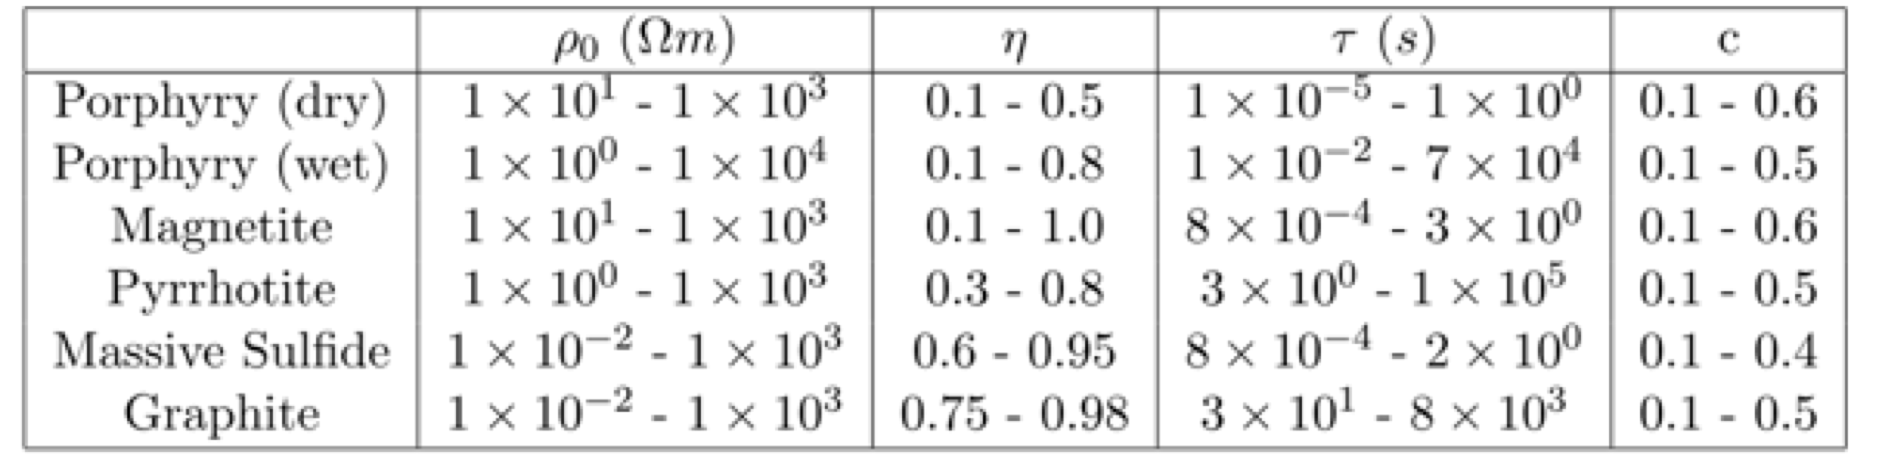
\includegraphics[width=0.8\textwidth]{figures/tablerocks.png}
  \caption{Cole-Cole parameters from different rocks (obtained from \cite{Pelton1978}).}
  \label{Fig:tablerocks}
\end{figure}

IP surveys have been successfully conducted in various geoscience applications. For mining applications, IP surveys are recognized as a principal geophysical technique for finding disseminated sulfide or porphyry deposits. This is mainly because of the metallic polarization effects arising from metallic minerals such as pyrite. On the other hand, non-metallic polarization effects (e.g. membrane polarization) can generate IP signals in various geological settings. Based on that, IP surveys have been used  in a broad spectrum of environmental problems including hydraulic conductivity estimation and hydrocarbon contaminant mapping \cite[]{Kemna2012}. 

A common type of IP survey is a DCIP survey where current electrodes, connected to a generator, are used to inject currents into the earth (galvanic source) and potentials are measured at potential electrodes. For time domain measurements, the input current waveform has an  on- and off-time (half-cycle rectangular waveform) as shown in Fig. ~\ref{Fig:IPonoff}. At the  potential electrodes on the surface, we measure a potential difference while input currents are on and off. Fig. ~\ref{Fig:IPonoff} shows measured voltage, and here $V_s$ indicates the secondary voltage (off-time), $V_0$ and $V_{\infty}$ are potential differences at zero and infinite frequency, respectively. 
\begin{figure}[htb]
  \centering
  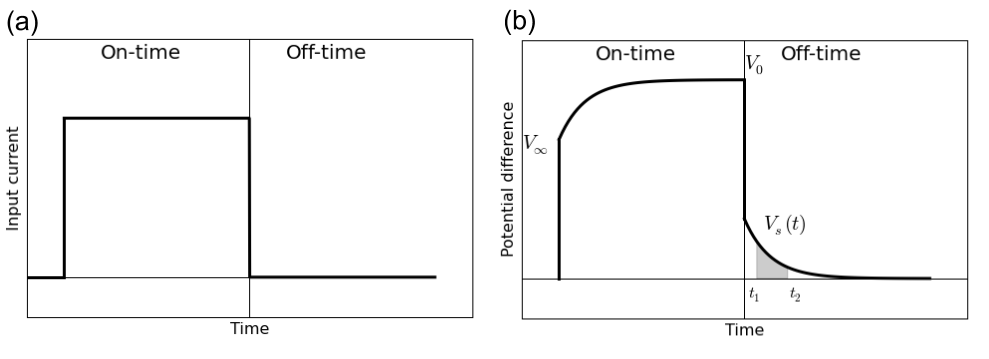
\includegraphics[width=0.8\textwidth]{figures/IPonoff.png}
  \caption{Conceptual diagram of (a) half-cycle input current waveform and (b) measured IP responses at surface electrodes.}
  \label{Fig:IPonoff}
\end{figure}
Assuming there are no EM induction effects, any signal in the off-time is the result of IP phenomena. Hence, any datum that captures some aspect of this secondary voltage is considered to be an IP datum. A most used form of the time domain IP data, $\dip$ can be written as  
\begin{equation}
  \dip = \frac{1}{V_0}\int_{t_1}^{t_2} V_s(t)
\end{equation}
Here $t_1$ and $t_2$ are arbitrary times included in the off-time when $t_1 < t_2$. When IP data correspond to the area of shaded region in Fig. ~\ref{Fig:IPonoff},  its unit is ms. However, each time channel of secondary potential can be considered as an IP datum, then the units of $\dip$ can be mV/V. In the frequency domain, since measured voltage is complex-valued, both amplitude and phase are considered as $\dip$ data. Assuming we have measured voltage at two different frequencies, percentage frequency effect (PFE), and phase difference (mrad), are also commonly used as $\dip$ data.  

Interpretation of the IP data is most commonly carried out by taking one of the many definitions of IP data (mV/V, ms,pfe, mrad), assume that chargeability is small, linearize  the problem \cite[]{seigel1959}, and invert to find 2D or 3D volumes of a chargeability \cite[]{doug1994}. 
This IP inversion is commonly carried out using a two-stage inversion procedure: a) first recover a resistivity distribution at zero frequency from DC data (latest on-time data or lowest frequency), then b) recover a chargeability distribution by inverting $\dip$ data using a sensitivity function from the previous DC inversion.

Not all chargeable volumes are the economic resources sought and it is desirable to distinguish between the different chargeable units. Determining different IP characteristics by interpreting multiple time and frequency channels has thus been a long term goal. The generic term for this study is spectral IP (SIP). For instance, we may want to differentiate between a porphyry and a magnetite embedded in the earth. Both of them have significant chargeability, but different time constants as shown in Fig. ~\ref{Fig:tablerocks}. By inverting SIP data, and recovering both chargeability and time constants we could possibly differentiate between those two different rocks. 

A simple and most often used approach is to invert each time or frequency IP data separately, and then interpret the recovered models to distinguish different IP sources using a complex resistivity model \cite[]{Yuval1997,Kemna2004,Hordt2006}. 
More sophisticated approaches invert multiple time or frequency IP data simultaneously by parameterizing the complex resistivity model with a few parameters e.g. Cole-Cole \cite[]{Kemna2004,Fiandaca2012}. Either approach can provide distributed IP information that is insightful. A principal challenge for inverting SIP data in 3D space is the increased dimensionality due to frequency- or time-dependent resistivity. For instance, in the frequency domain, the output of the inversion can be $\rho(x,y,z;\omega)$. This is four-dimensional function. Even if we parameterize complex resistivity, $\rho(x,y,z;\omega)$  using the Cole-Cole model, which is a simple complex resistivity model, we still have four times the number of parameters to be solved  because of the four Cole-Cole parameters: $\rho_0$, $\eta$, $\tau$, $c$. 
With the first approach where each time or frequency is inverted separately, this dimensionality issue may not be a critical problem. However, for the second approach where all parameters are found at once, one needs an effective strategy to handle increased dimensionality to proceed successful 3D inversion. Considering this generic challenge for inverting SIP data, we chose the first approach to recover 3D distribution of IP parameters. 

A significant assumption behind the interpretation of DCIP data is ignoring EM induction effects. Depending on both the resistivity of the earth and measured times or frequencies, there can be a number of situations where this assumption is not reasonable. For several decades, this issue has been treated using EM decoupling techniques; that is, use a  method to remove EM induction effects from the observations and thereby extract IP signals. There have been various EM decoupling techniques suggested based on approximate representations of EM induction effects using a half-space or layered-earth resistivity model \cite[]{Wynn1975,routh2001}. Although they have been effective for some case histories, I believe that we have to revisit the EM decoupling issue using our 3D forward modelling and inversion capabilities.  

On the other hand, whenever an electric field is applied to the earth, IP signals can be generated from a chargeable body. Thus, not only galvanic sources, but also inductive sources such as airborne loop transmitters can excite chargeable bodies. However, the electric field generated by an inductive source is solely based on EM induction, and hence it is fundamentally different from the galvanic source excitation. This difference needs to be considered in order to proceed to the interpretations of inductive source IP (ISIP) data. The airborne time domain IP problem is at the leading edge for geophysics research. Negative transients measured in coincident loop data are commonly observed \cite[]{SmithandKlein,JansenEtAl2004,Kang2015b}. Such negatives can only be explained by having an earth that is chargeable \cite[]{Weidelt1982}. Inverting these ISIP data, and recovering IP parameters, may yield information about near surface structure that is relevant to mineral exploration and/or environmental problems such as permafrost \cite[]{SmithandKlein, Kang2015b}. These ISIP data have typically been inverted by invoking a half-space or layered-earth assumption \cite[]{Kratzer2012}. Yet IP signals are small and 3D analysis is likely necessary for many problems. Therefore, recovering 3D information of IP parameters from ISIP data is an important topic. 

In my Ph.D. research, I will focus on interpreting time domain IP data from both galvanic and inductive sources. My goal is recover  3D distributions of IP parameters, such as Cole-Cole parameters, and use that information to  distinguish different rock units  as magnetite and porphyries. 
At this point, I plan to  adopt the two-stage approach \cite[]{doug1994}, but modify it to handle both EM effects and be able to extract more IP parameters. The techniques will be applicable to inductive and galvanic sources in the ground, on the earth’s surface, or in the air.  Two main items to be tackled in my Ph.D research are:  a) designing an effective EM decoupling procedure to remove EM induction effects from the data, and b) develop a sensitivity function and a strategy to carry out 3D IP inversion for ISIP data. In the next section, to identify both EM induction and IP effects, I perform forward modelling with a single galvanic source with multiple receivers. 

%% =============================================================================
%% Sub section. Complex resistivity
%% =============================================================================

\subsection{Complex resistivity}

Mathematical representations of these IP effects are often defined in the requency domain with the resistivity represented as a complex function.
An extremely simple, but a most used model, is called the Cole-Cole model. One representation due to  \cite{Pelton1978} can be expressed as 
\begin{equation}
  Z(\omega) = R_0 \Big[1 - \eta \Big(1-\frac{1}{1+(\imath\omega\tau)^c}\Big) \Big],
  \label{eq:colecole}
\end{equation}
where $R_0$ is resistance at zero frequency, $\eta$ is chargeability, $\tau$ (s) is a time constant, $c$ is a frequency dependency. As frequency goes to infinity, the above complex impedance value ($Z(\omega)$) asymptotes to $R_{\infty} = \frac{R_0}{1-\eta}$. This yields an expression of the chargeability as 
\begin{equation}
  \eta = \frac{R_0-R_{\infty}}{R_0}.
\end{equation}
Complex resistivity, $\rho(\omega)$ can be simply obtained by 
\begin{equation}
  \rho(\omega) = Z(\omega)\frac{A}{l},
\end{equation}
where $A$ and $l$ are area (m$^2$) and length (m) of a sample rock. 

%% =============================================================================
%% Sub section. Lab scale IP measurments
%% =============================================================================

\subsection{Lab scale IP measurements}
To understand how IP effects can be measured, we consider a lab-scale IP measurement system used in Geological Survey of Canada \cite[]{Enkin2012} as shown in Figure ~\ref{Fig:instrumentIP}. A core sample cut in a standardized size and shape is located between two cylinder-shaped copper electrodes. To prevent possible charge build-up on contacts of electrodes and rock, two papers, soaked with copper sulphate, were attached between the rock sample and copper electrodes. A transmitter and a volt-meter are attached to the copper electrodes. The transmitter generates sinusoidal current ranging from 0.025Hz -1MHz, and the volt-meter measures the complex impedance at each transmitting frequency. 
\begin{figure}[htb]
  \centering
  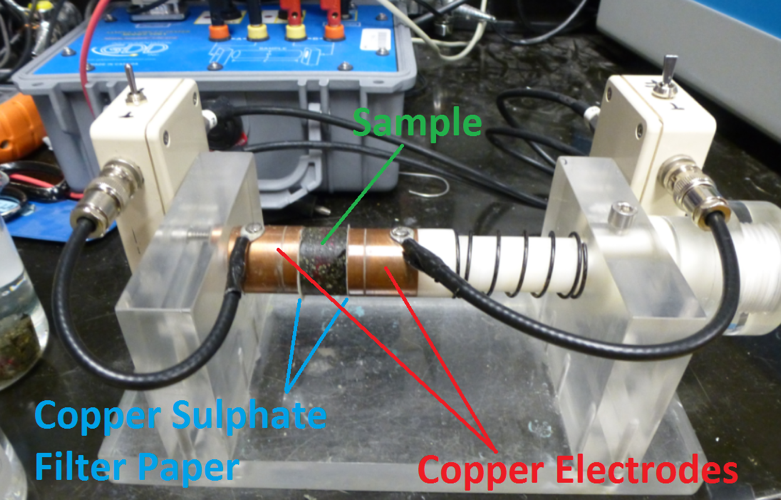
\includegraphics[width=0.5\textwidth]{figures/instrumentIP.png}
  \caption{Lab scale IP measurement system in Geological Survey of Canada (GSC). }
  \label{Fig:instrumentIP}
\end{figure}

Fig. ~\ref{Fig:obsimpedance}(a) shows the measured complex impedance from a core sample obtained from Highland Valley region of British Columbia, Canada. This is a porphyry deposit. The black solid lines show the observed amplitude and phase of the measured impedance. The observations are assumed to be the sum of a complex impedance associated with the rock as well as other instrument effects such as capacitive effects associated with the copper electrodes and electrode effects associated with the contacts between the copper sulfate paper and rock. The black dots are the predicted data associated with all of these effects. The contribution to the complex impedance that arises from the rock is provided by the ``star''. This is the response of a Cole-Cole model, with parameters shown on the plot.  For further details about extracting the impedance of the rock from the observations, the reader is referred to see \cite{Enkin2012}. The Cole-Cole impedance reproduces the lower and mid-frequency of the observations. The chargeability of the porphyry is estimated to be $\eta=0.16$ and the time constant $\tau=2.6\times10^{-3}$s. 

 %The low frequency data can be fit with a Cole-Cole model  and dots show the observed and predicted complex impedances, respectively. Complex impedances closely related to instrumentations: are effectively considered for this set-up to fit the observed impedances.  Recovered Cole-Cole parameters correspond to rock are also shown on the left panel of Fig. ~\ref{Fig:obsimpedance}(a). 

 As a second example, I present the complex impedance of a core sample obtained from the Tli Kwi Cho kimberilte complex. It is shown in Fig. ~\ref{Fig:obsimpedance}(b). This sample shows significantly different Cole-Cole parameters especially for the time constant ($\tau$). For the kimberlite $\tau \simeq 4\times10^{-5}$s which is very small compared to that from the porphyry deposit. This difference may be due to different polarization mechanisms. The first sample from a porphyry deposit contains significant amount of pyrites which are possibly more related to metallic polarization. On the other hand, the sample from the kimberlite deposit (crater facies) contains a considerable amount of clay minerals and hence membrane polarization might be dominant. However, the exact understanding for the cause of the IP response is not crucial for my research. What is important is that in a lab scale, these two rocks are associated with different IP parameters.  A geophysical experiment that captures the IP signature of rocks may thus allow us to distinguish between them. 

\begin{figure}[htb]
  \centering
  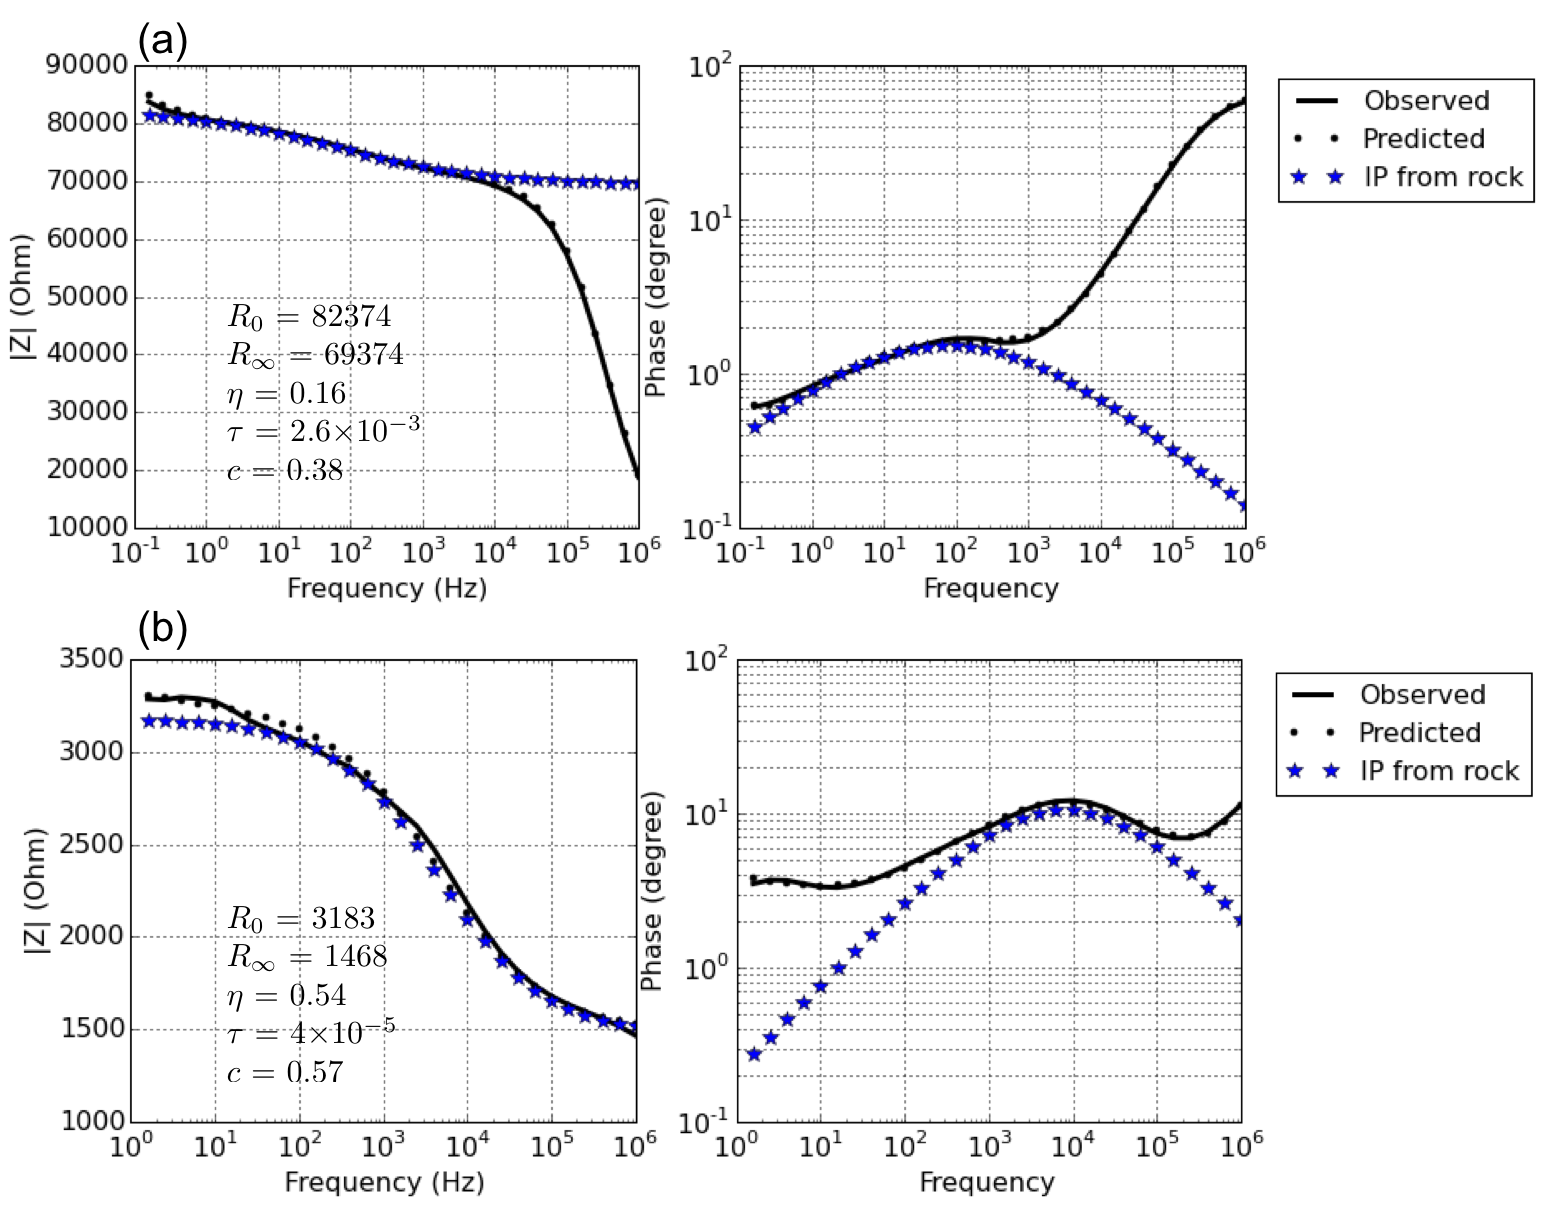
\includegraphics[width=0.8\textwidth]{figures/obsimpedance.png}
  \caption{Complex impedance measurment system in Geological Survey of Canada \cite[]{Enkin2012}. }
  \label{Fig:obsimpedance}
\end{figure}
\clearpage

%% =============================================================================
%% Sub section. Modelling Maxwell's equations
%% =============================================================================

\subsection{Modelling Maxwell's equations}
IP responses in various types of time domain electromagnetic (TEM) surveys are governed by Maxwell’s equations. Different from usual case, conductivity of the earth is frequency or time-dependent. In general, similar to the complex resistivity shown in Eq. \ref{eq:colecole}, complex conductivity in frequency domain can be defined as 
% Seogi: we may need to comment the reason why we prefer conductivity to resistivity (?)
\begin{equation}
  \sigma(\omega) = \siginf + \dsig(\omega),
  \label{eq:sigmaomega}
\end{equation}
where $\siginf$ is conductivity at infinite frequency.
In time domain this can be expressed as
\begin{equation}
  \sigma(t) = \siginf\delta(t) + \dsig(t),
  \label{eq:sigmat}
\end{equation}
where $\delta(t)$ is Dirac-Delta function. For a specical case when Cole-Cole model with $c$=1, $\dsig(\omega)$ can be expressed as 
\begin{equation}
  \dsig(\omega)= -\sigma_{\infty}\frac{\eta}{1+(1-\eta)(\imath\omega\tau)},
\end{equation}
In time domain, $\dsig(t)$ can be expressed as 
\begin{equation}
  \dsig(t)=-\siginf\frac{\eta}{(1-\eta)\tau}e^{-\frac{t}{(1-\eta)\tau}}.  
\end{equation}

I set electromagnetic (EM) fields without IP effects as fundamental fields, and corresponding Maxwell’s equations can be written as 
\begin{equation}
  \curl \e^{F} = -\frac{\partial \b^{F}}{\partial t},
  \label{eq: eq_primary_farad}
\end{equation}
\begin{equation}
  \curl{\frac{1}{\mu}\b^{F}} -\siginf\e^{F} = \j_s.
  \label{eq: eq_primary_coulomb}
\end{equation}
Here superscript $F$ on EM fields in above equations mean fundamental fields, $\e$ is the electric field ($V/m$), $\b$ is the magnetic flux density ($Wb/m^2$), $\j_{s}$ is the current source ($A/m^2$) and $\mu$ is the magnetic permeability ($H/m$).
Observed data will include both EM and IP effects, and corresponding Maxwell’s equations can be written as
\begin{equation}
  \curl{\e} = -\frac{\partial \b}{\partial t},
  \label{eq: total_farad}
\end{equation}
\begin{equation}
  \curl{\frac{1}{\mu}\b} - \sigma(t)\otimes\e(t)= \j_{s},
  \label{eq: total_coulomb}
\end{equation}
where $\otimes$ indicates time convolution for a causal signal. Note that total current $\j$ is a convoltion of $\sigma(t)$ and $\e(t)$ due to time-dependent conductivity. 
Theses observed EM fields can be defined as $\e = \e^{F} + \e^{IP}$, $\b = \b^{F} + \b^{IP}$ and $\j = \j^{F} + \j^{IP}$, where superscript $IP$ is induced polarization. 

Simply, IP response, $\dip$ can be computed as 
\begin{equation}
  \dip(t) = F[\sigma(t)] - F[\siginf] = d-d^F
\end{equation}
where $F[\cdot]$ is Maxwell's operator, which outputs arbitrary EM fields with input conductivity model. Observed and fundamental resposnes correspond to $d=F[\sigma(t)]$ and $d^F=F[\siginf]$, respectively. 
The above subtraction corresponds to the EM decoupling \cite[]{Pelton1978,routh2001}. By solving both Maxwell’s equations we can evaluate observed and fundamental responses, which allows us to comptue $\dip$. For these simulations I use EMTDIP code developed by \cite{Marchant2014}. 

To understand how both fundamental and IP fields behave in a TEM survey, I consider a simple grounded TEM survey, which has a single transmitter. Current waveform includes 2100 ms on- and off-time, and in on-time current flows in counter-clockwise direction. Fig. ~\ref{Fig:chargmodel} shows a transmitter wire path and the chargeability distribution in the core region of the 3D mesh (except padding cells). The chargeability of the chargeable block is 0.1. The distribution of the conductivity model at the infinite frequency is set to half-space model of which conductivity ($\sigma_{half\text{-}space}$) is 0.05 S/m. I run two forward modellings corresponds to the observed ($d=F[\sigma(t)]$) and the fundamental ($d^F=F[\siginf]$) responses then obtain $\dip$ by subtracting $d^F$ from $d$. Computed potential difference with these set-ups at two electrode locations (marked as black dots in Fig. ~\ref{Fig:chargmodel} (a) are shown in Fig. ~\ref{Fig:DecayFullResis}. Right after the current switch-on, there are significant induced EM responses, then as time goes later those EM responses decay and the observed responses converge to the steady-state. Here I provide the normalized potential difference, which means $V(t)/V_0$, where $V(t)$ is the observed potential difference and $V_0$ is the one at the DC limit. This often considered as the DC datum. After the current switch-off (often called off-time), there are significant EM induction, and this decays as time passes. Fig ~\ref{Fig:EvecResisfull}(a) and (b) show plan and section views of the electric fields, respectively at the 6 (the top panel), 715 (the middle panel), and 2116 (the bottom panel) ms. These three times are marked as the black solid lines in Fig. ~\ref{Fig:DecayFullResis}. At the 6 ms, we can clearly recognize the induced EM signals from the current wire path, and those disappear as time goes later which asymptotes to the DC limit. 

\begin{figure}[htb]
  \centering
  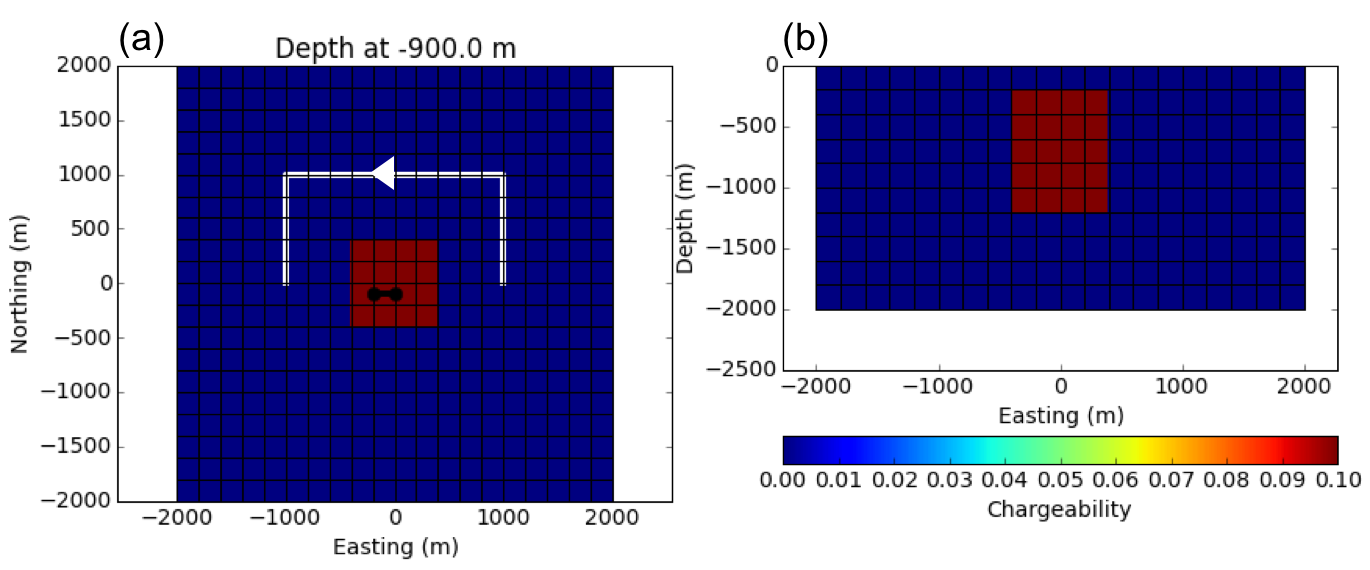
\includegraphics[width=0.6\textwidth]{figures/chargmodel.png}
  \caption{3D chargeability model. (a) Plan and (b) Secion views. White solid line on (a) shows current wire path, and arrow indicated direction of the current at on-time. }
  \label{Fig:chargmodel}
\end{figure}

\begin{figure}[htb]
  \centering
  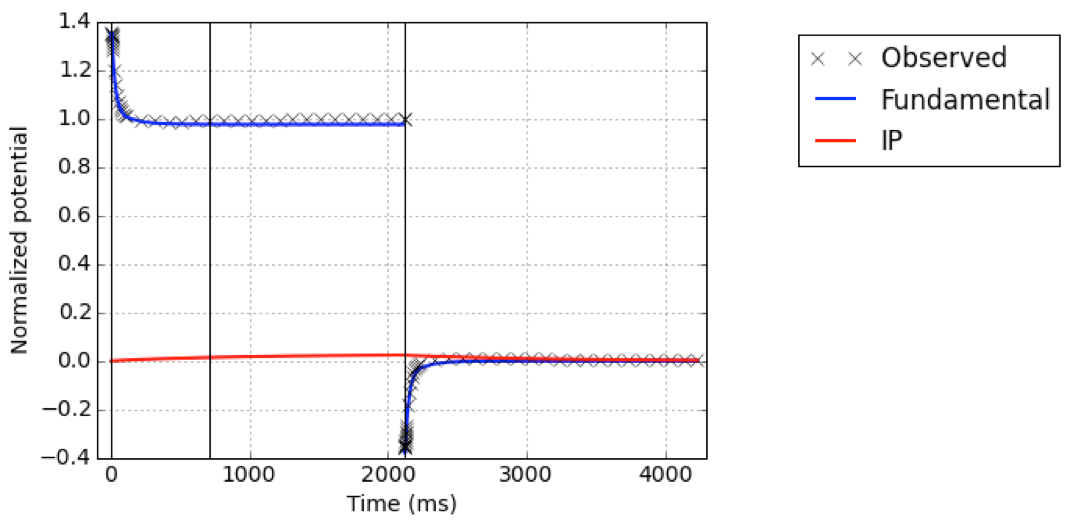
\includegraphics[width=0.6\textwidth]{figures/DecayFullResis.png}
  \caption{Time curves of the normalized potential difference at a receiver location (marked as black solid line with dots in Fig. ~\ref{Fig:chargmodel}(a)). Cross marks, blue line, and red line correspondingly indicate observed, fundamental and IP data. Black solid lines at three times indicate times we provided electric field distribution at Fig. ~\ref{Fig:EvecResisfull}}
  \label{Fig:DecayFullResis}
\end{figure}

\begin{figure}[htb]
  \centering
  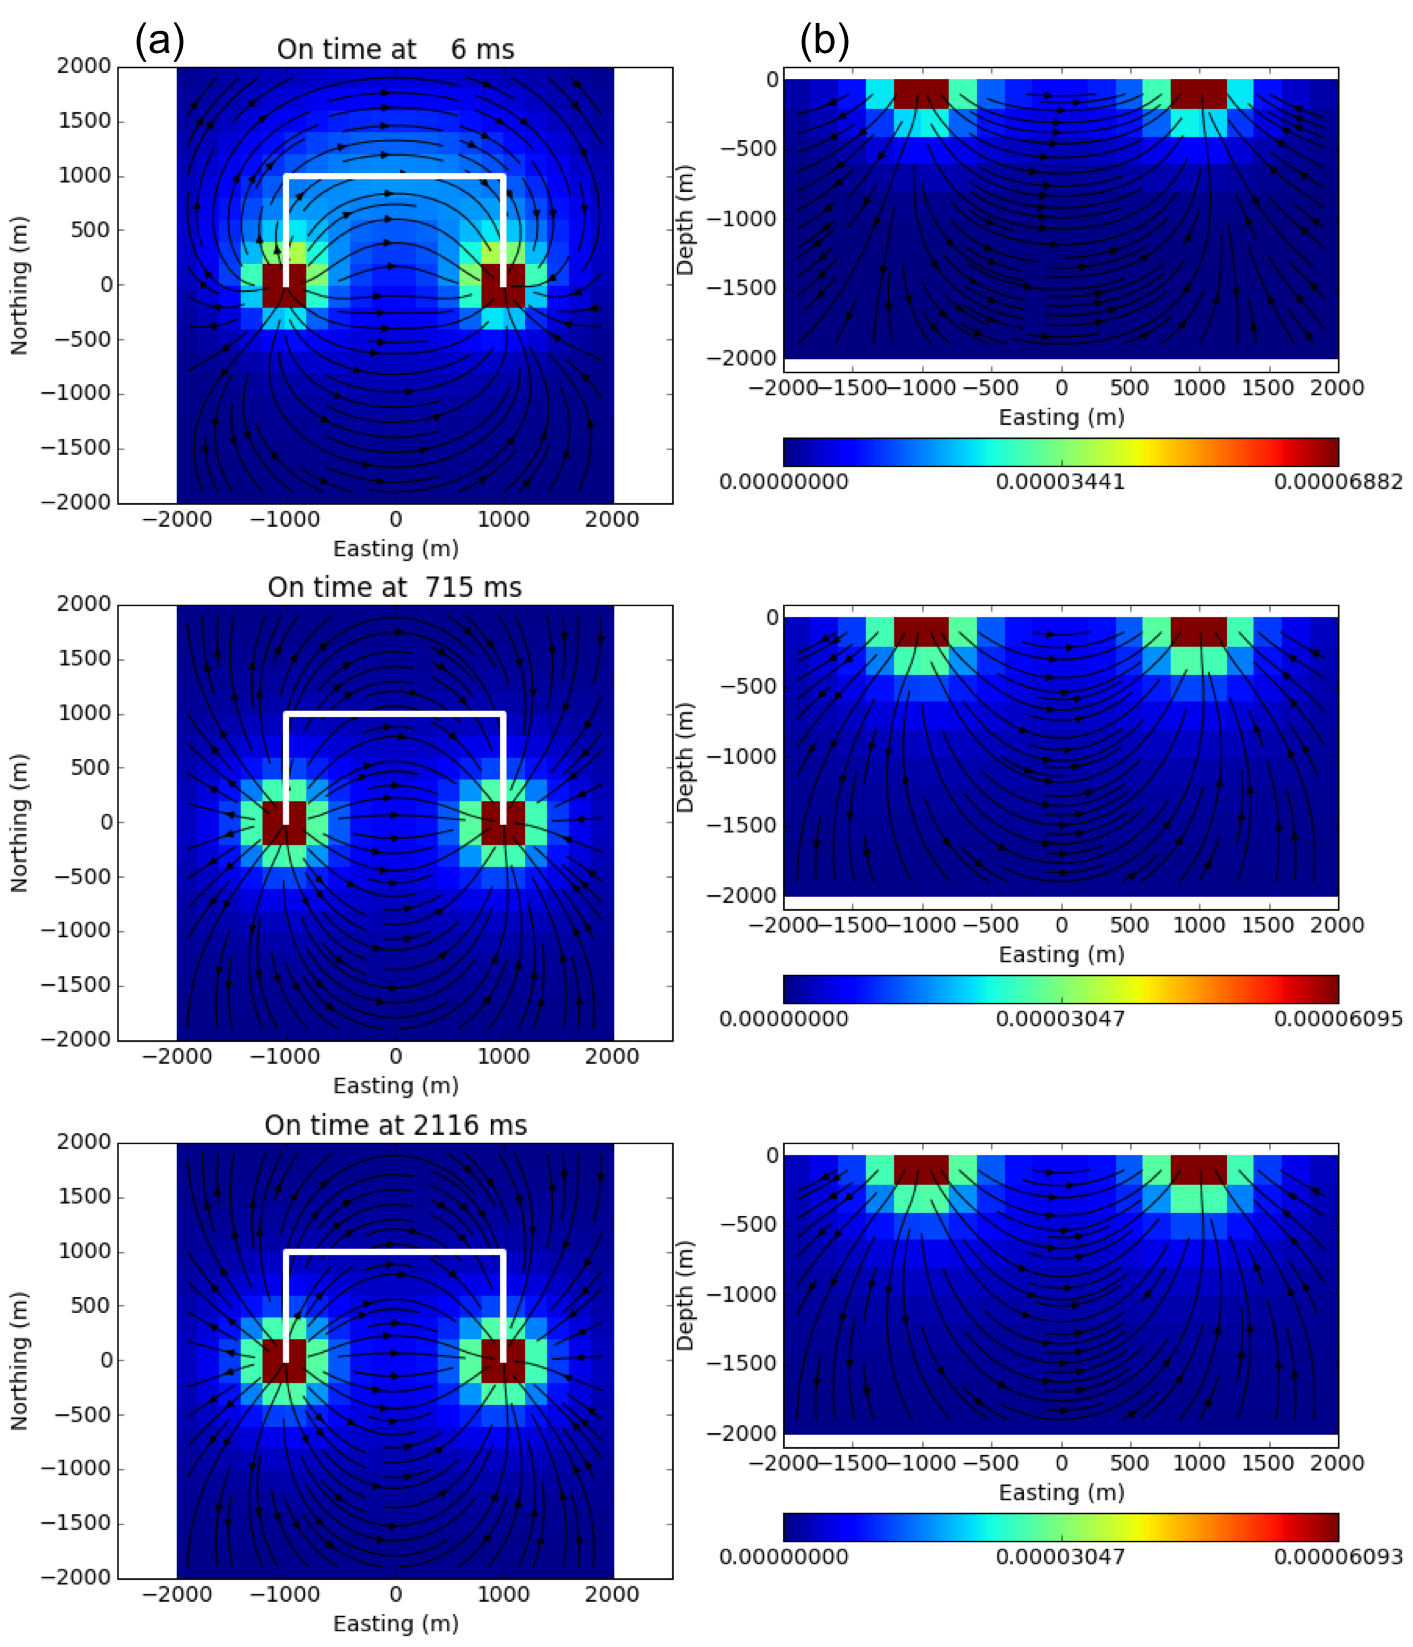
\includegraphics[width=0.6\textwidth]{figures/EvecResisfull.png}
  \caption{3D electric field distribution at three different times in the on-time. Top, middle and bottom panel correspondingly show electric fields at 6, 77, and 1717 ms. (a) Plan and (b) Secion views. }
  \label{Fig:EvecResisfull}
\end{figure}

In the on-time, IP responses (red line) are much smaller than fundamental responses (blue line), whereas in the off-time the IP responses could be considerable enough to be identified. Fig. ~\ref{Fig:DecayOffResis} show only off-time signals in the form of log-scaled normalized potential. Note that ``off-time'' means the time after we off the input current, and I set that time as our zero time (0 ms). Dotted and solid lines differentiate the sign of responses. At the early times ($\sim$ 10 ms), observed and fundamental responses are almost coincident because EM induction is dominant at this time. As we move to the later time, relative strength of the IP is increasing, and at the $\sim$ 500 ms IP is dominant. Fig ~\ref{Fig:EvecResisoff} shows the electric fields at three off times (6, 77, and 1717 ms). Significant EM induction effect is observed at the 6 ms near the current wire. This EM field significantly decayed at the 77 ms, which has smooth distribution except for the chargeable region. At 1717 ms, the IP field is dominant, and the chargeable body acts as a dipole. 
In addition, the measured potential difference (Easting direction) on the surface are shown in Fig ~\ref{Fig:RespResisoff} at the corresponding three off times. 

\begin{figure}[htb]
  \centering
  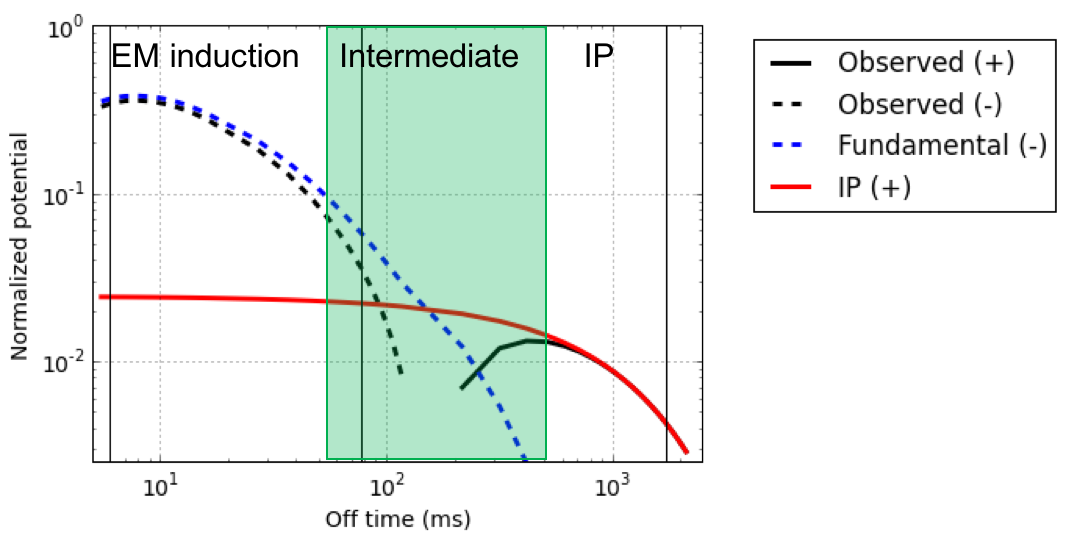
\includegraphics[width=0.6\textwidth]{figures/DecayOffResis.png}
  \caption{Time decaying curves of the normalized potential difference at the off-time. Black, blue, and red line correspondingly indicate observed, fundamental and IP data. Dotted and solid lines distinguish postive and negative values. Black solid lines at three times indicate times I provided electric field distribution at Fig. ~\ref{Fig:EvecResisoff}}
  \label{Fig:DecayOffResis}
\end{figure}

\begin{figure}[htb]
  \centering
  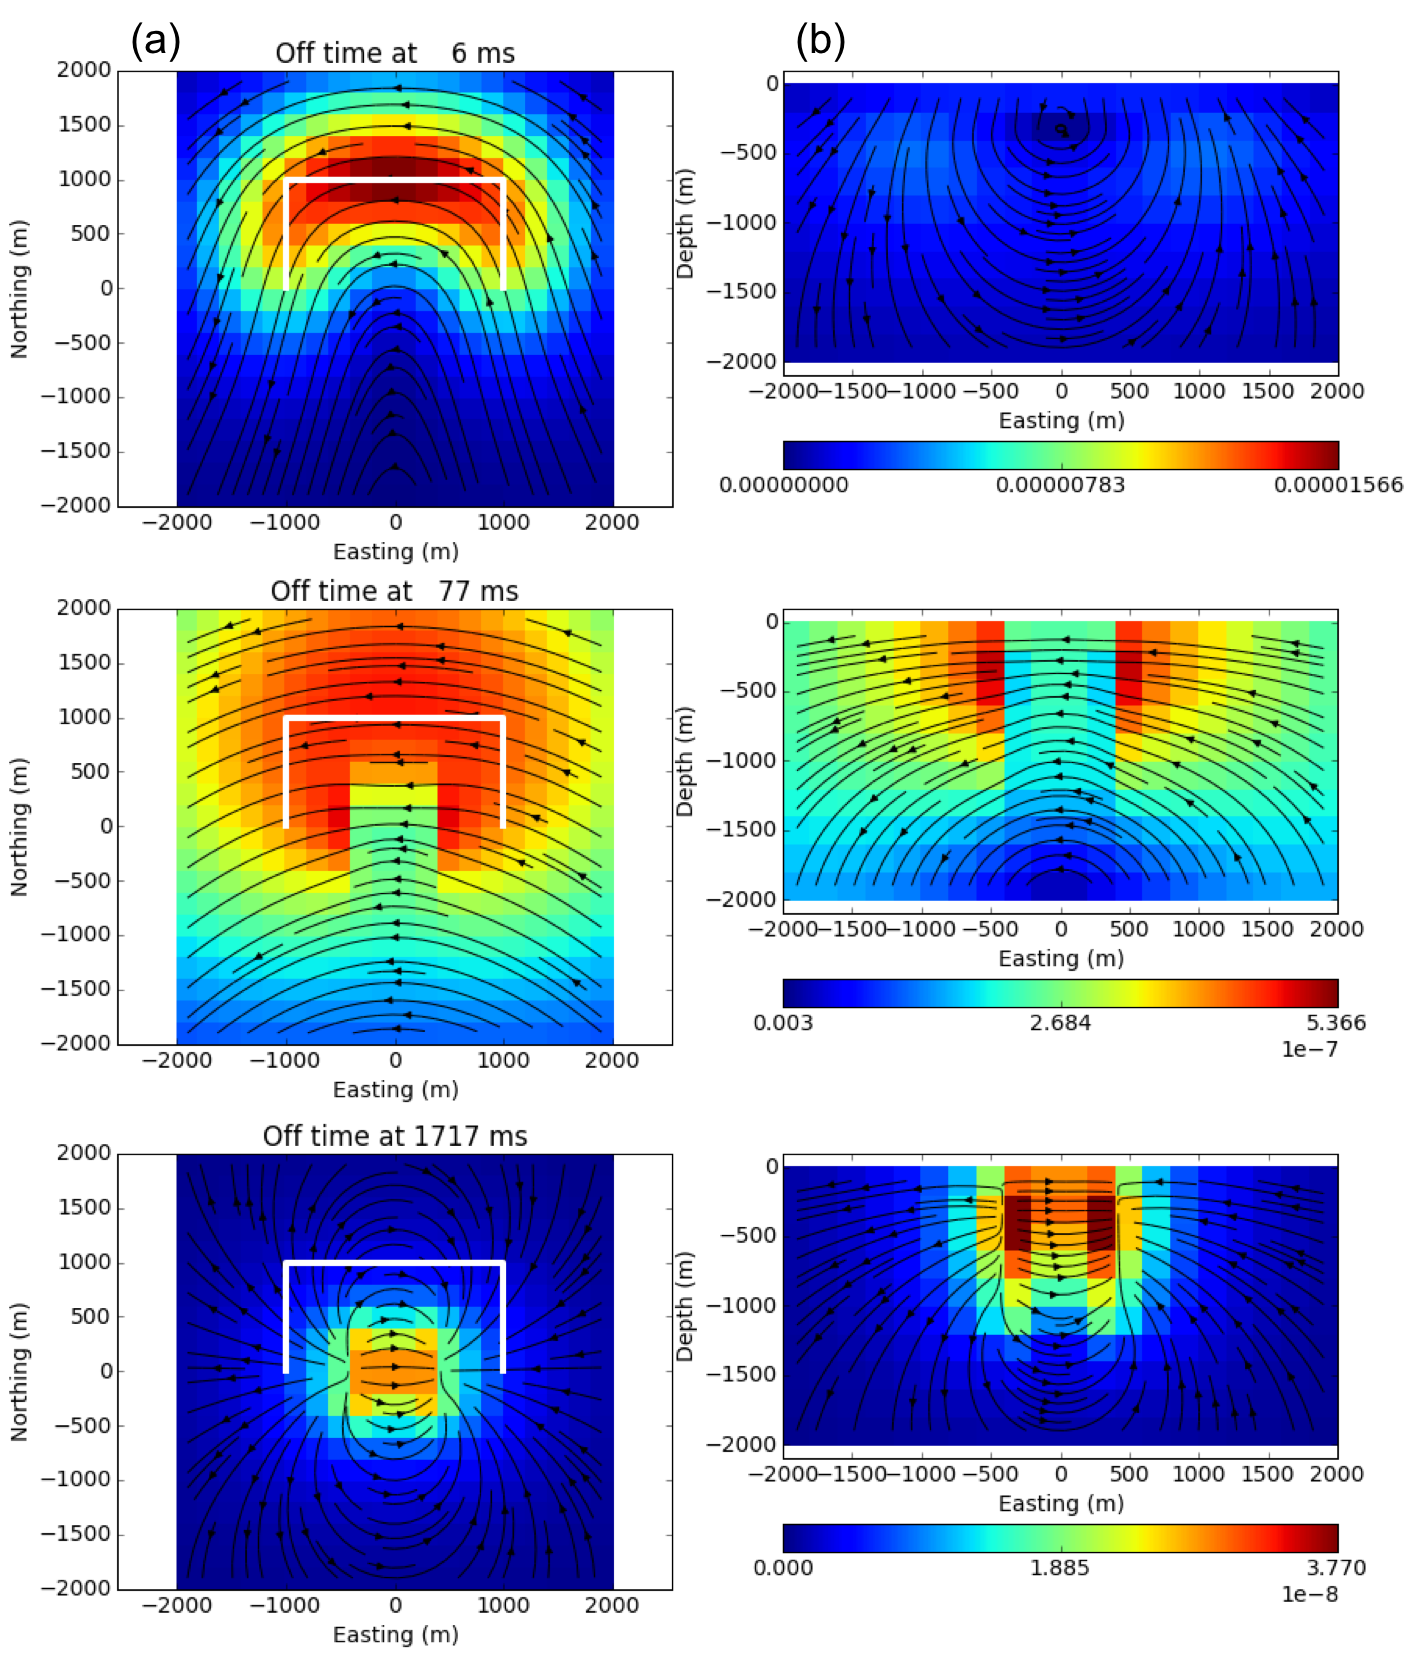
\includegraphics[width=0.6\textwidth]{figures/EvecResisoff.png}
  \caption{3D electric field distribution at three different times in the off-time. Top, middle and bottom panel correspondingly show electric fields at 6, 715, and 2116 ms. (a) Plan and (b) Secion views.}
  \label{Fig:EvecResisoff}
\end{figure}

\begin{figure}[htb]
  \centering
  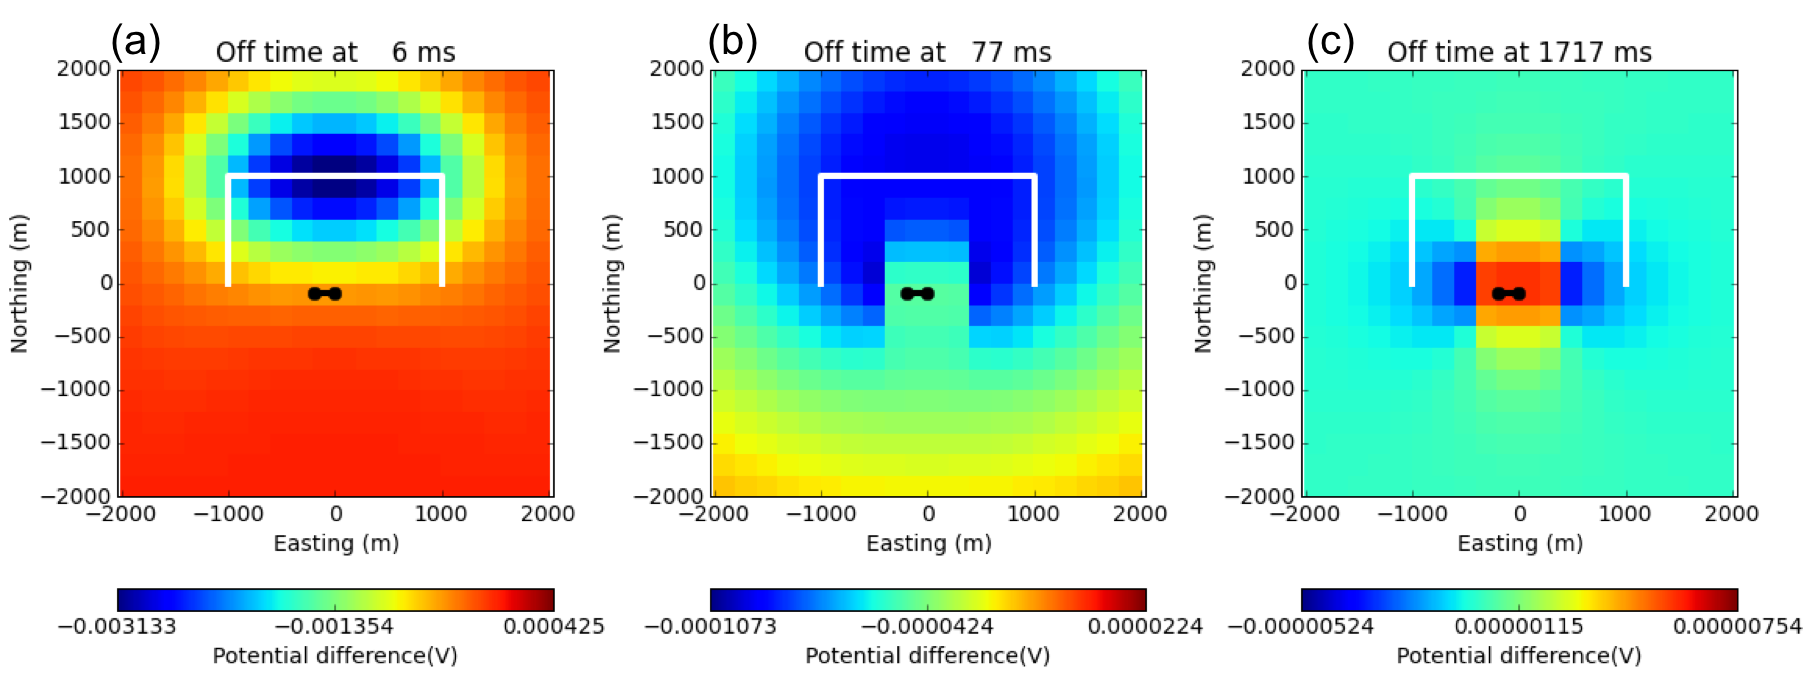
\includegraphics[width=0.8\textwidth]{figures/RespResisoff.png}
  \caption{Observed potential difference at three different off times. (a) 6 ms, (b) 77 ms, and (c) 1717 ms. }
  \label{Fig:RespResisoff}
\end{figure}

Most of time domain IP surveys assume that they are in the IP dominant time, which is reasonable for the resistive earth. 
However, for the conductive earth, this assumption could break. To see the effects of the conductive earth in the observed data, I only increase $\sigma_{half-space}$ as 0.5 S/m (ten times greater than previous example). Fig ~\ref{Fig:DecayFullCond} shows the normalized potential at both on- and off-time channels. Compared to the previous resistive example, this shows much slow variation of the responses in time resulting in slower converges of them to the steady-state (DC limit). As shown in Fig ~\ref{Fig:DecayOffCond}, fundamental responses at off-time show the sign reversal at $\sim$ 20 ms. Even at the late times $\sim$ 1000 ms the IP response is much smaller than the fundamental response. Fig ~\ref{Fig:RespCondoff} shows the measured potential difference on the surface at the same three times (6, 77, and 1717 ms). 

\begin{figure}[htb]
  \centering
  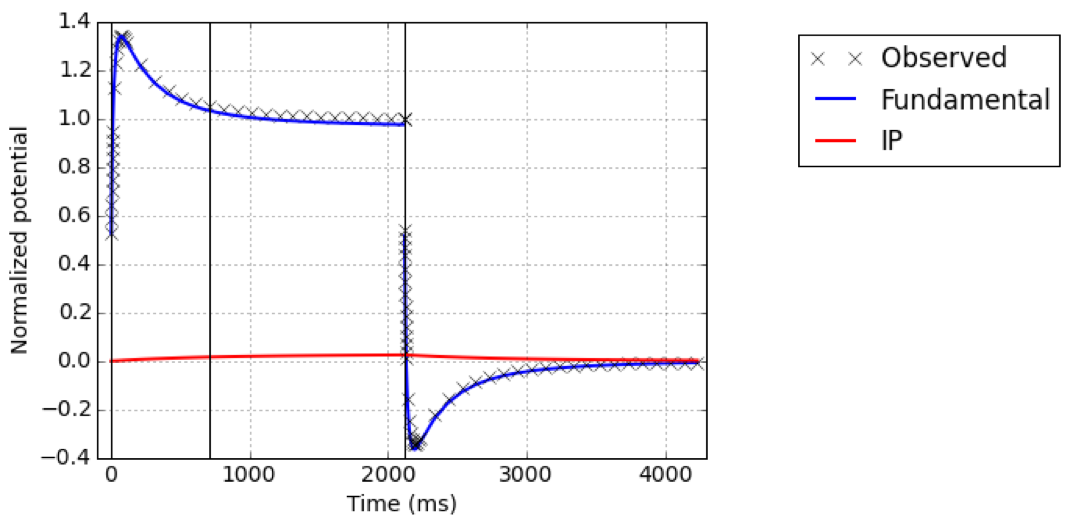
\includegraphics[width=0.6\textwidth]{figures/DecayFullCond.png}
  \caption{Time curves of the normalized potential difference at a receiver location (marked as black solid line with dots in Fig. ~\ref{Fig:chargmodel}(a)). Half-space conductivity of this model is increased to 0.5 S/m compared to Fig. ~\ref{Fig:DecayFullResis}.}
  \label{Fig:DecayFullCond}
\end{figure}

\begin{figure}[htb]
  \centering
  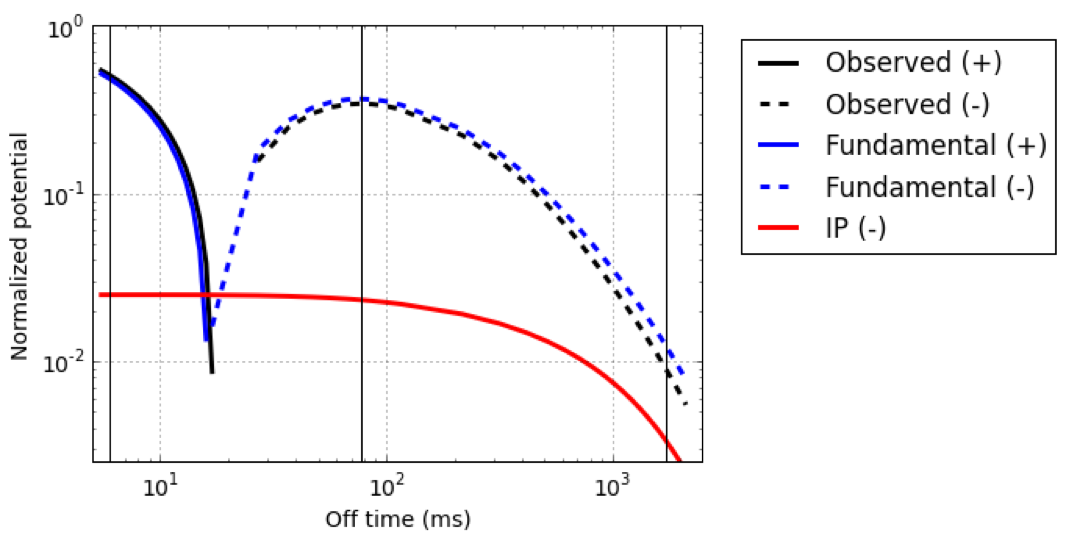
\includegraphics[width=0.6\textwidth]{figures/DecayOffCond.png}
  \caption{Time decaying curves of the normalized potential difference at the off-time. Half-space conductivity of this model is 0.5 S/m to Fig. ~\ref{Fig:DecayOffResis}.}
  \label{Fig:DecayOffCond}
\end{figure}

\begin{figure}[htb]
  \centering
  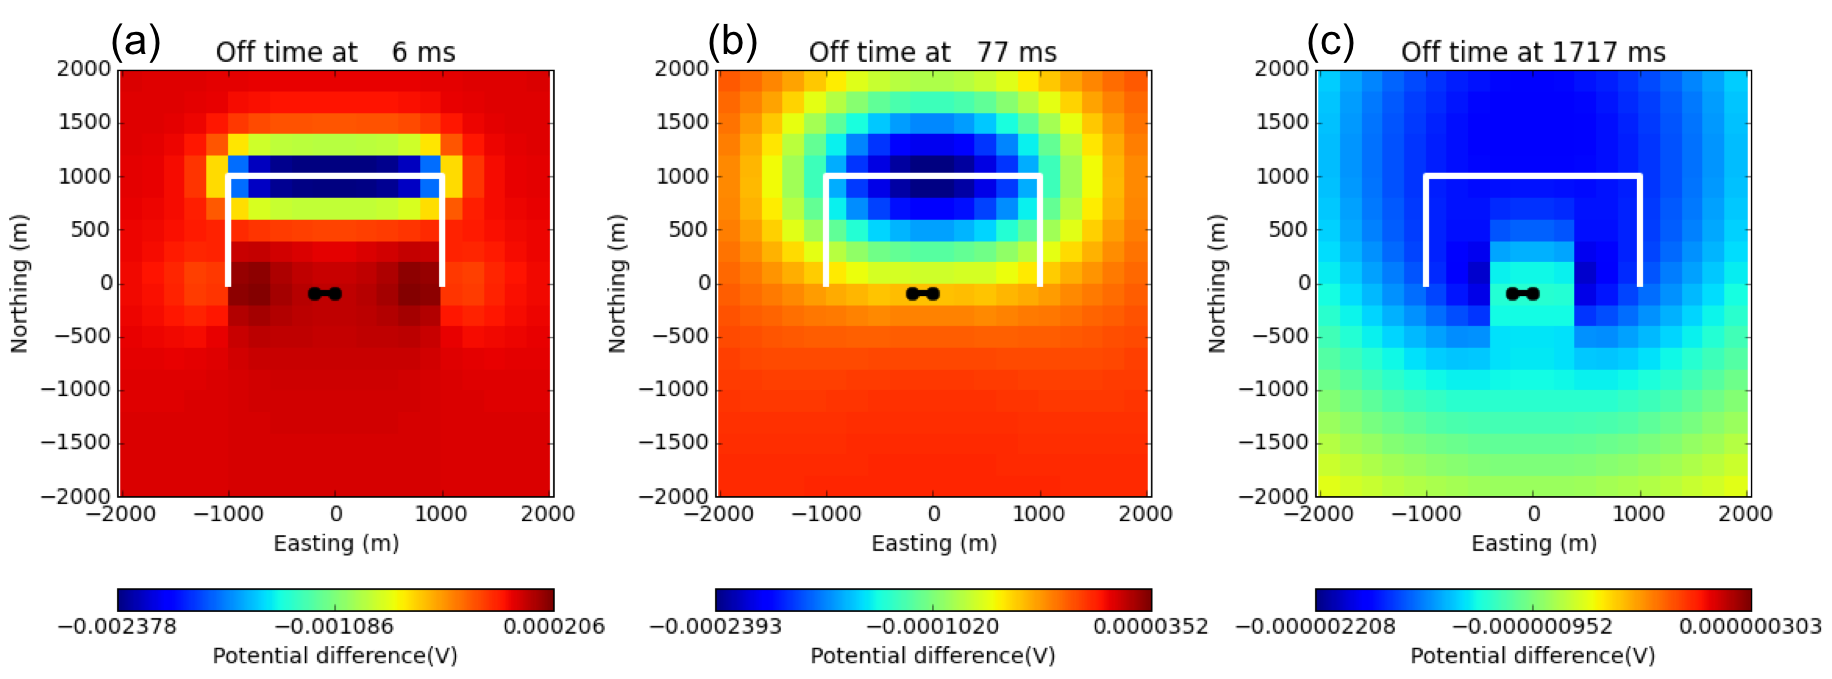
\includegraphics[width=0.8\textwidth]{figures/RespCondoff.png}
  \caption{Observed potential difference at three different off times. (a) 6 ms, (b) 77 ms, and (c) 1717 ms. Half-space conductivity of this model is 0.5 S/m to Fig. ~\ref{Fig:RespResisoff}.}
  \label{Fig:RespCondoff}
\end{figure}

To summarize, in the observed responses there can be natural separation of EM and IP responses in time as shown in Fig. ~\ref{Fig:DecayOffResis}:
\begin{itemize}
  \item at the early time: EM-dominant
  \item at the intermediate time: Both EM and IP are considerable
  \item at the late time: IP-dominant
\end{itemize}
At the EM-dominant time, IP is minor so that I could use these EM responses to recover the conductivity distribution, thus I want to remove the IP-coupling as much as I can. However, at the IP-dominant time, the EM induction effect is minor thus, I want to remove the EM coupling to restore the chargeability distribution.  
\clearpage

\section{STRATEGIES OF RECOVERING DISTRIBUTED IP INFORMATION}
My final goal is to recover distributed IP information from TEM data. To achieve this goal, I need to pose a proper problem, and effective strategies. There can be three main options that I could use to achieve this goal. 

The first is to formulate the inverse problem to find a complex conductivity. In the frequency domain, I can apply a separate inversion for each frequency and recover a complex conductivity distribution \cite[]{Kemna2004,commer2011}. In the time domain, I can parameterize complex conductivity as few parameters (e.g. Cole-Cole: $\siginf$, $\eta$, $\tau$, and $c$), then jointly invert for those multiple parameters \cite[]{Fiandaca2012,Marchant2013,Xu2013}. Especially for the 3D inversion, this will increase both the non-uniqueness and the computational cost of the inversion dramatically hence, I do not choose this option. 

The second option is to realize that the signal has an early (EM) part, a late (IP) part and an intermediate zone of mixed signals as shown in Fig. ~\ref{Fig:DecayOffResis}. Isolate these by applying EM decoupling or IP decoupling, and work with each independently. This is what has been done with most routine applications \cite[]{doug1994}. For instance, the two-stage approach inverts on-time data to recover the conductivity and uses that conductivity to invert off-time data to recover the chargeability. Although the two-stage inversion approach is robust and cost-effective, this will have issues when the earth is considerably conductive due to the remaining EM induction effects at the ``late enough times''. 
I prefer this approach to the first one mostly due to its robustness and cost-effectiveness. However, I want to treat possible EM-coupling in the off-time data. 

% Although simultaneous 3D inversions considering both EM induction and IP effects might be an attractive option to interpret time domain IP data, still we believe there are some major challenges for this approach to be established as a robust technique. 
% Two main issues in this simultaneous inversions are a) resolvability of EM induction and IP effects in the inversion and b) increased non-uniqueness due to frequency-dependent resistivity. 


Accordingly, I adopt the two-stage approach and develop a linearized formulation to solve for a pseudo-chargeability. The first step  is to estimate a background conductivity. To achieve this, I  can invert the late on-time data using the DC inversion algorithm or the early off-time data using the TEM inversion algorithm. Either way, a selection of data for inversion assumes that any IP effects on data are insignificant. Using the estimated conductivity, I can  forward model the TEM response; this is an approximate fundamental response. By subtracting this from the observation, I define the IP datum, and this corresponds to EM decoupling. I thenuse a linearized approach to recover a pseudo-chargeability by inverting those IP data. 

\section{SPECTRUM OF RESEARCH PROBLEMS}
The physics behind build-up for polarization charges only requires that we have an electric field of sufficient strength and duration so that that the polarization currents are built up. Hence, the same phenomenon will happen with galvanic or inductive sources. The only difference is the exact form of the electric field. Fig. ~\ref{Fig:singlpixelE}(a) and (b) shows the fundamental electric field at a single pixel in the earth for the galvanic and the inductive sources, respectively. However, detailed implementations of my two-stage IP inversion approach will be different. In order to treat complications due to different excitation mechanisms and survey set-ups, I consider three different geophysical surveys:
\begin{itemize}
  \item Grounded sources with many receivers
  \item Single inductive source with many receivers
  \item Multiple inductive sources with a single receiver for each source (airborne TEM)
\end{itemize}

My goal is to develop a comprehensive inversion workflow to invert  these three types of surveys. Thus far I have concentrated upon the most difficult one (first item) because it is new and potentially important. 

The workflow for the airborne IP inversion is shown in Fig. ~\ref{Fig:workflow}. Different from DCIP data, airborne IP data does not have any steady-state electric field that we can simply invert using the DC inversion algorithm. Accordingly, I first invert early time TEM data, recover a 3D conductivity assuming IP effects in this data are minor. Second, using that conductivity model, I forward model the TEM data, subtract those from the observation, and obtain the IP data. Because the estimated conductivity model is not exact, there can be possible residual field. If this residual field is composed of mostly long wavelength spatial components, I can fit them using a low order polynomial and remove them, which is common in magnetic problem (regional removal). With consideration of this residual field, our EM decoupling procedure can be formulated as 
\begin{equation}
  \dip_{raw}(t) = d(t) - d[\sigma_{est}](t) = \dip(t) + \triangle d[\siginf](t) + n(t),
  \label{eq: IPdatum_raw}
\end{equation}
where $\dip$ is the true IP data, $n$ is the additive noise, and $\triangle d[\siginf]$ ($=d^{F}-d[\sigma_{est}]$) is the error caused because of poor estimate of $\siginf$. 
The observed IP datum after residual removal procedure can be written as 
\begin{equation}
  \dip_{obs}(t) = \dip_{raw}(t) - \triangle d_{est} = \dip(t) + \triangle d[\siginf](t) + n(t) - \triangle d_{est}(t),
  \label{eq: IPdatum_obs}
\end{equation}
where $\triangle d_{est}(t)$ is estimated residual field. 
In order to invert this observed IP datum, I use a linearized approach. Different form of the electric field for the inductive source is effectively incorporated in our linear sensitivity function \cite[]{Kang2015c}. Final form of the linear equation can be written as 
\begin{equation}
  \dip(t) = G\peta(t),
  \label{eq:linearIPdatum}
\end{equation}
where $G$ is the sensitivity function, and $\peta(t)$ is pseudo-chargeability. Using this linear kernel, I separately apply 3D IP inversion to $\dip_{obs}(t)$ and recover $\peta(t)$ at each time channel. Finally by interpreting inversion outputs at multiple time channels I estimate the Cole-Cole, or equivalent IP parameters. For further details of our methodology see Section \ref{section:appendix}

\begin{figure}[htb]
  \centering
  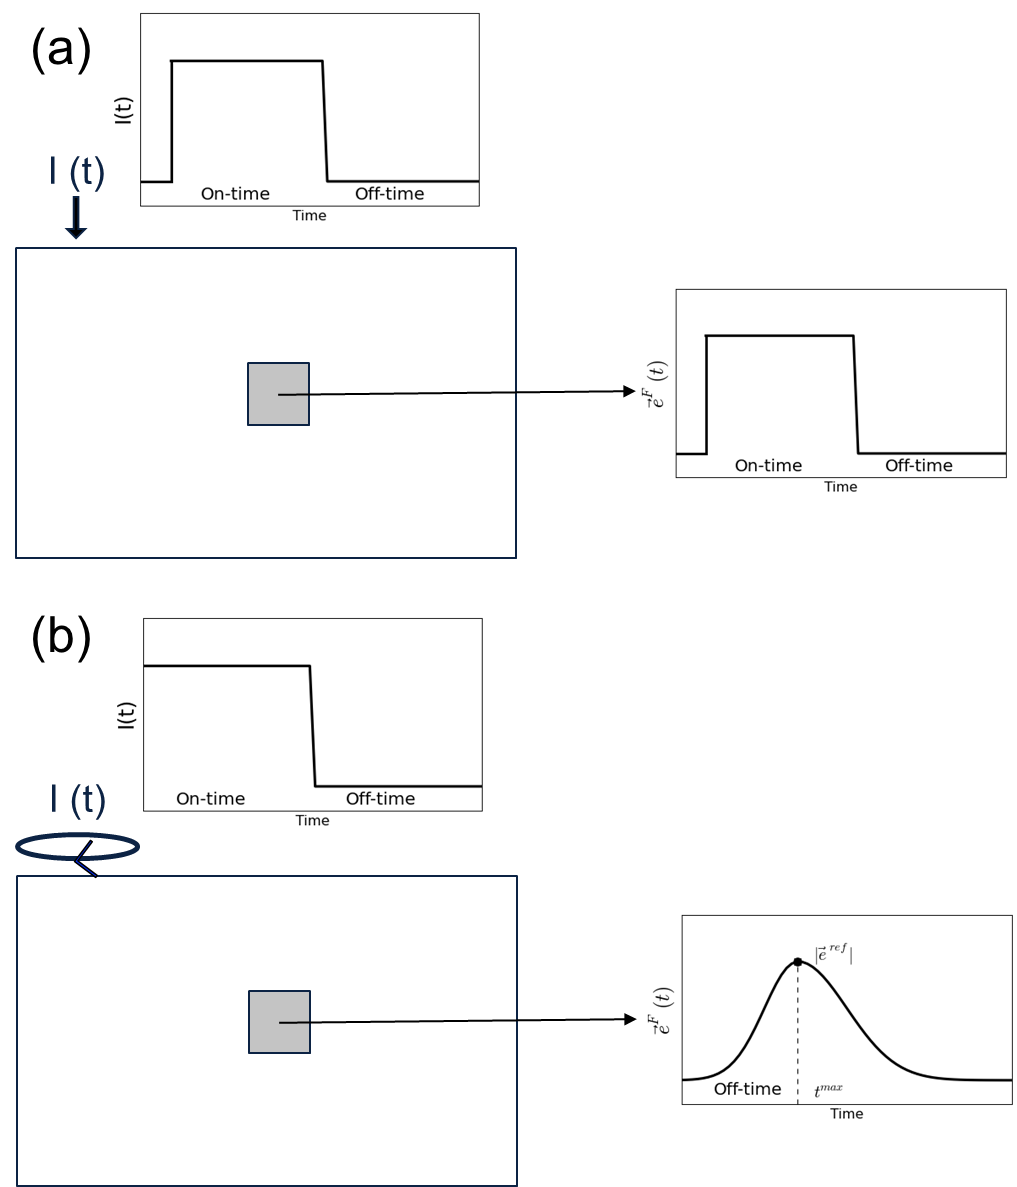
\includegraphics[width=0.5\textwidth]{figures/singlpixelE.png}
  \caption{Time behaviour of fundamental electric field at a single pixel in the earth due to the input current. (a) Galvanic source and (b) Inductive source. }
  \label{Fig:singlpixelE}
\end{figure}

\begin{figure}[htb]
  \centering
  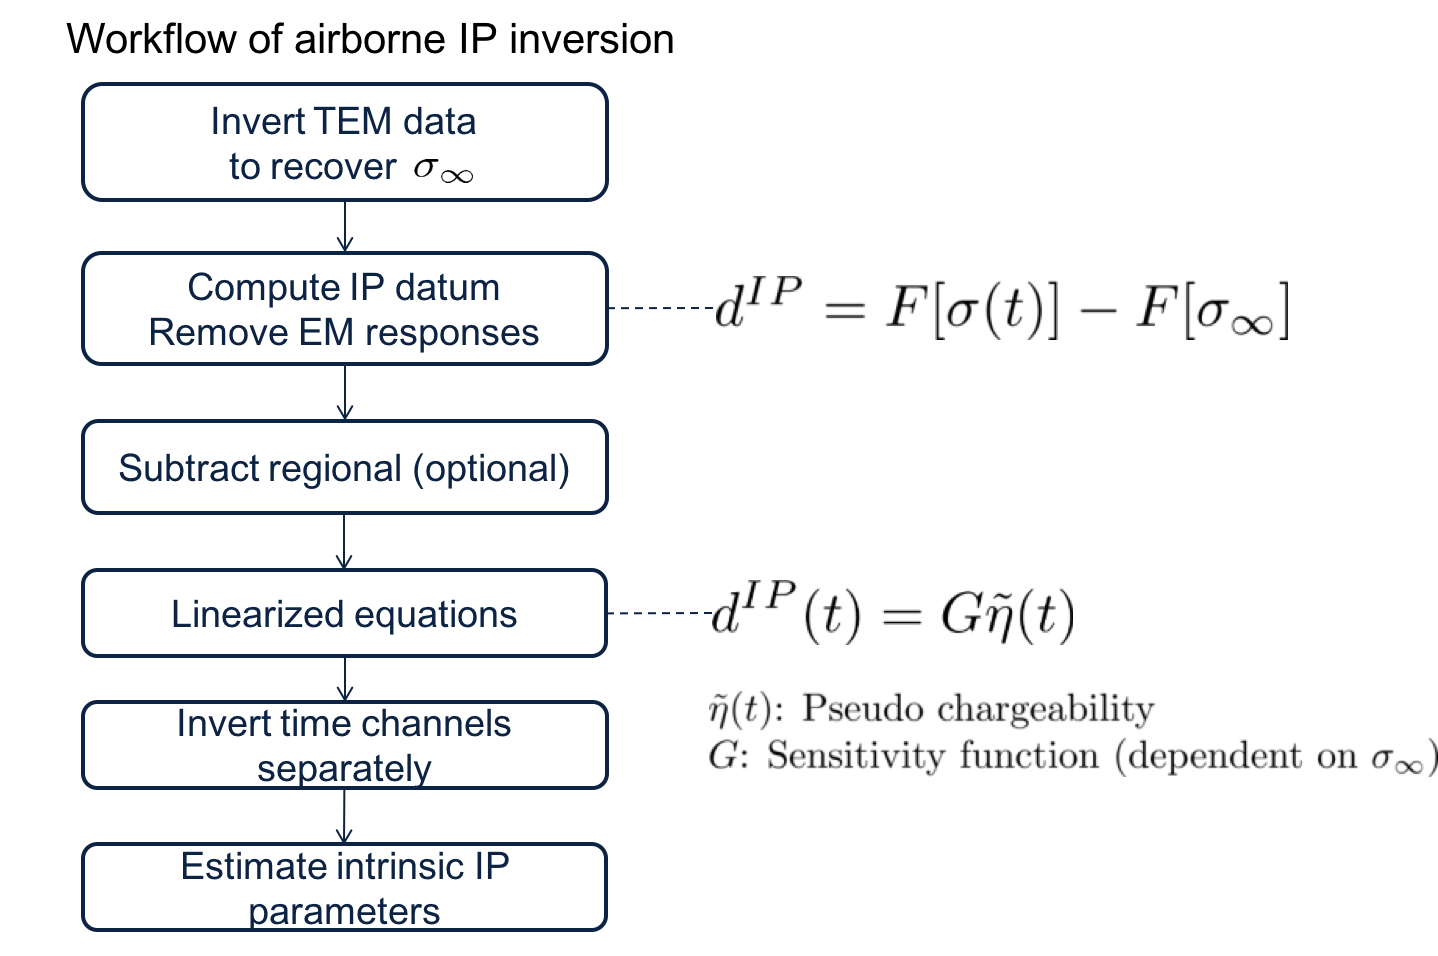
\includegraphics[width=0.8\textwidth]{figures/workflow.png}
  \caption{Work flow of the 3D airborne IP inversion. }
  \label{Fig:workflow}
\end{figure}
\clearpage

\section{EXAMPLE: TLI KWI CHO KIMBERLITE COMPLEX}
The Tli Kwi Cho (TKC) kimberlite complex is located approximately 360 km northeast of Yellowknife, NWT, Canada within the Archean Slave craton. The complex is part of the larger Lac de Gras kimberlite field, which hosts numerous diamondiferous kimberlites that make it of economic interest to the mining industry. Currently, there are three active diamond mines within 100 km of TKC: Snap Lake, Diavik, and Ekati. Today most of diamond exploration programs on Slave Craton are conducted with a combination of till sampling and airborne geophysics \cite[]{Pell1997}. Fig. ~\ref{Fig:tkcgeo}(a) shows standard kimberlite model composed of crater facies, diatreme facies, and hypabyssal facies. Kimberlites in Lac de Gras region mostly composed of crater and hypabyssal facies. Those facies are intruding granitic background. Both kimberlite facies have lower density than the granitic background. The crater facies usually has higher conductivity than the background due to the abundance of clay minerals. The hypabyssal facies has high magnetic susceptibility. From a geophysical prospecting point of view of TKC kimberlite, therefore we are looking for gravity low, magnetic high, and conductivity high. 

The TKC kimberlites are composed of two main pipes called DO-18 and -27 as shown in  Fig. ~\ref{Fig:tkcgeo}(b). There are four different kimberlites named XVK (Xenolithic kimberlite), VK (volcaniclastic kimberlite), HK (hypabyssal kimberlite) and PK (pyroclastic kimberlite). Corresponding region for each kimberlite is shown in Fig. ~\ref{Fig:tkcgeo}(b). DO-18 pipe is mostly XVK and DO-27 is a combination of PK and HK. An easting geological section at the DO-27 pipe generated from drilling results \cite[]{HarderEtAl2006} are shown in Fig ~\ref{Fig:tkcgeo}(c). 

Among several airborne geophysical surveys, I focus on an airborne TEM (ATEM) survey conducted VTEM system (Geotech Inc.). This system uses a coincident loop system where transmitting and receiving loops are colocated. For this specific case, in theory we cannot observe negative transients unless earth conductivity is time-dependent that is, earth is chargeable \cite[]{Weidelt1982}. In the VTEM data near DO-18 even at the earliest time channel (90 micro-s), negative transients were observed as shown in Fig ~\ref{Fig:TKCvtem}(a). Furthermore, the positive high anomaly near DO-27 at 90 micro-s (Fig. ~\ref{Fig:TKCvtem}(a)) changed to a  negative anomaly at 680 micro-s (Fig. ~\ref{Fig:TKCvtem}(b)). Although not shown here, observed AeroTEM data at TKC also show similar negative anomalies \cite[]{JansenEtAl2004}. Based on these observations, I believe that there are chargeable materials in TKC region, and the measured VTEM data includes that information. Myr goal is to apply our 3D airborne IP inversion procedure (Fig. ~\ref{Fig:workflow}), and recover distributed IP information at TKC region. I expect this chargeability information could be another physical property that could be used for kimberlite exploration in conjunction with density, magnetic susceptibility, and conductivity. 

\begin{figure}[htb]
  \centering
  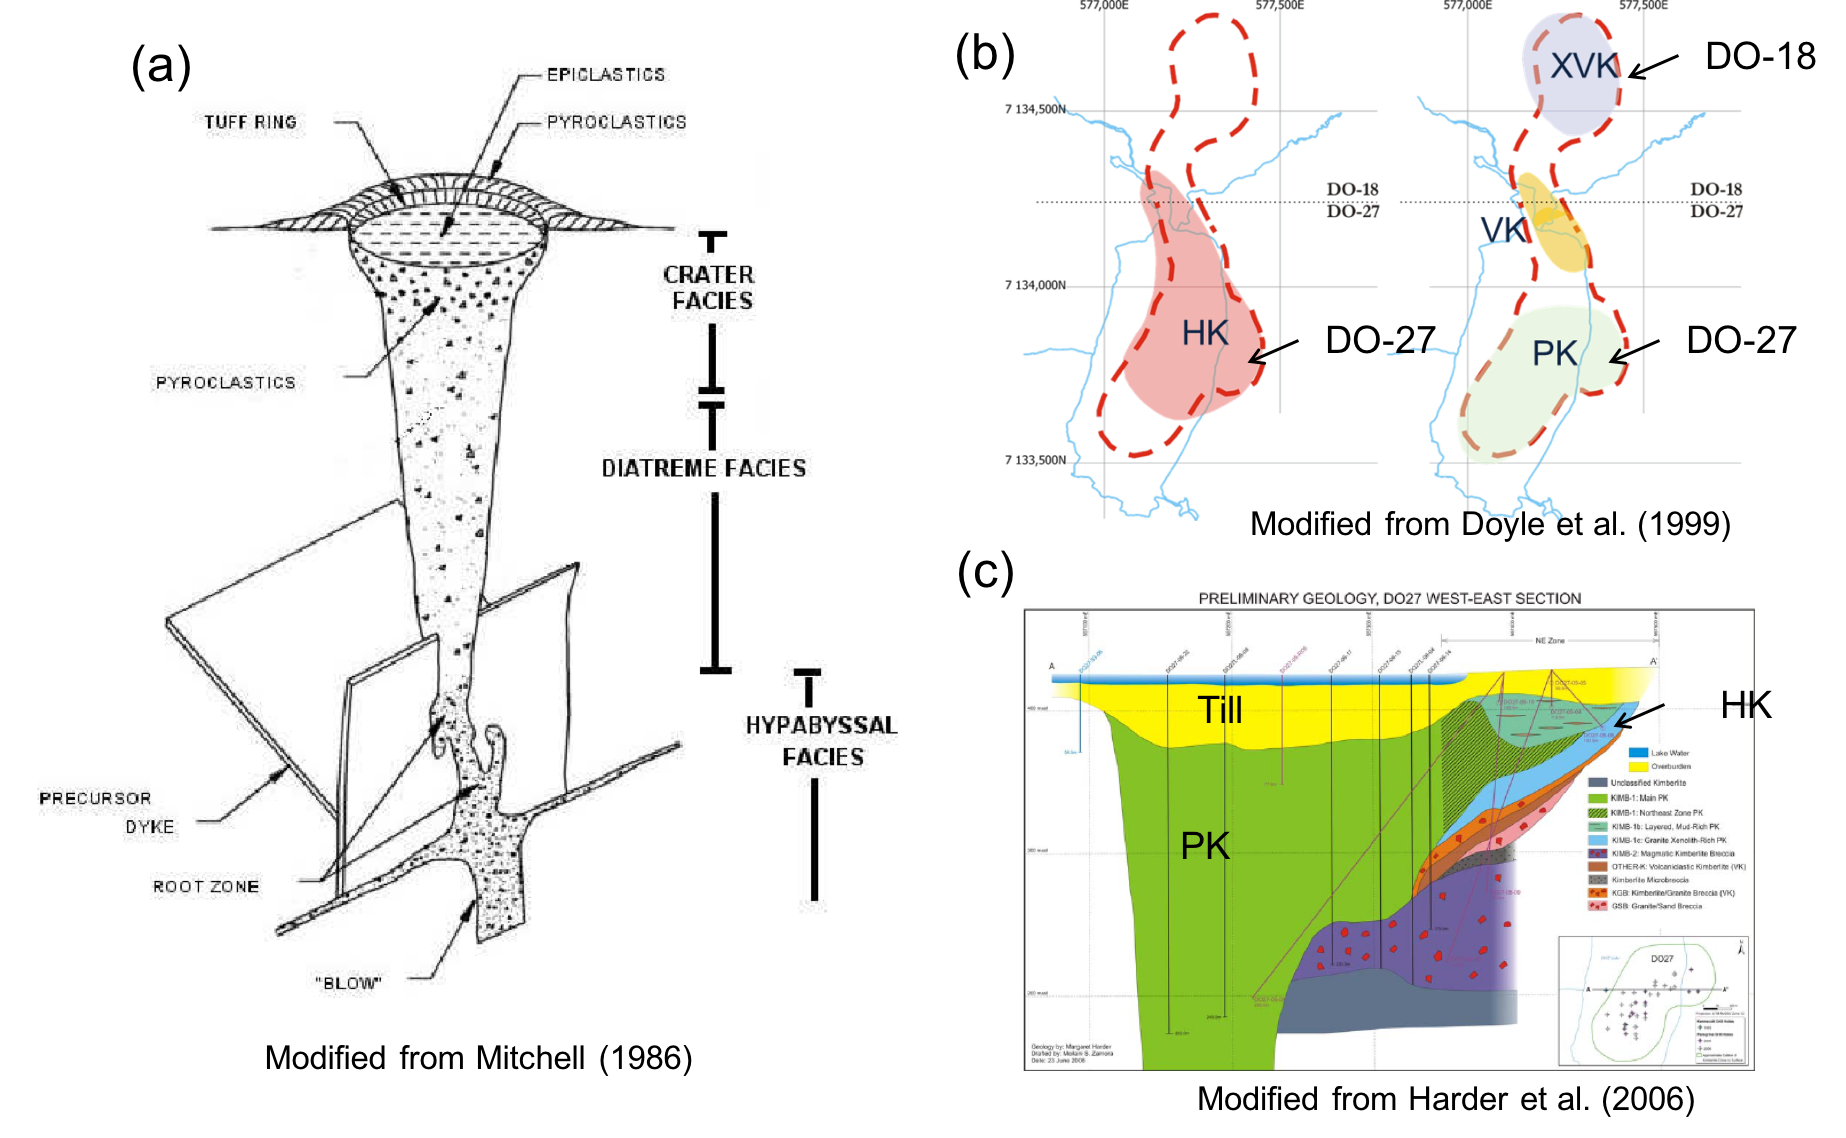
\includegraphics[width=0.8\textwidth]{figures/tkcgeo.png}
  \caption{(a) General kimberlite geology \cite[]{PowerHildes2007}. (b) Map of TKC region with four types of kimberlites: XVK, VK, HK, and PK (modified from \cite{JansenEtAl2004}). (c) Geoogical section at DO-27 (modified from \cite{HarderEtAl2006}). }
  \label{Fig:tkcgeo}
\end{figure}

\begin{figure}[htb]
  \centering
  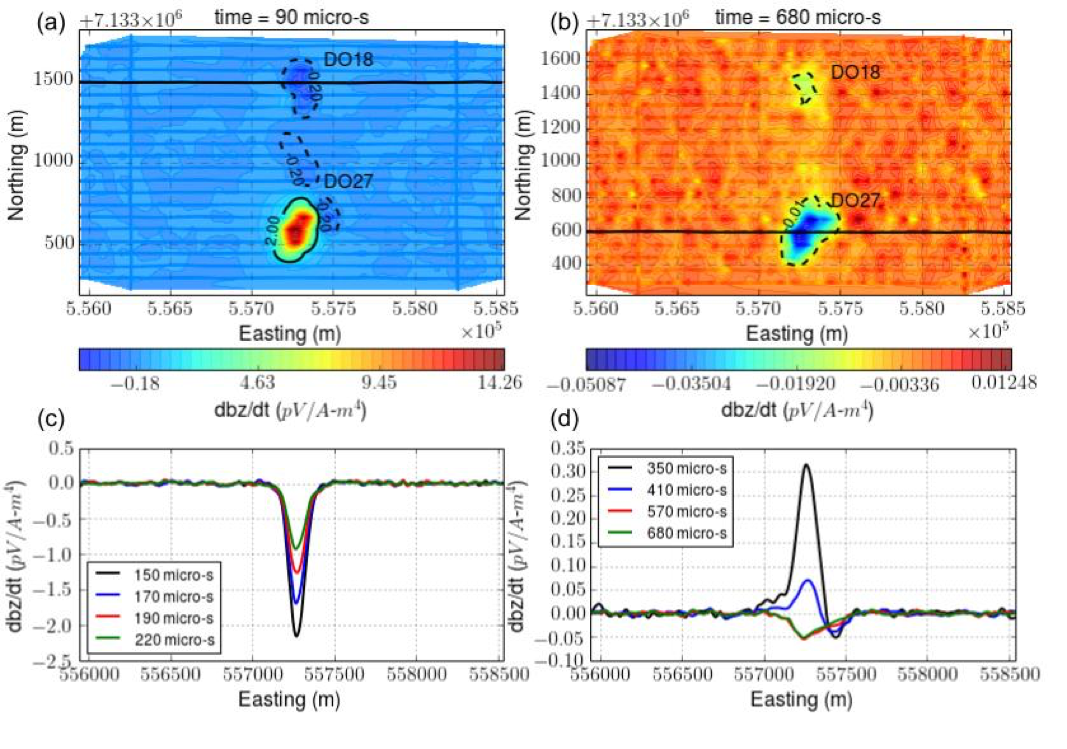
\includegraphics[width=0.8\textwidth]{figures/TKCvtem.png}
  \caption{TKC VTEM data. Maps of VTEM responses at (a) 90 micro-s and (b) 680 micro-s. Easting profile line data near (c) DO-18 and (d) DO-27. }
  \label{Fig:TKCvtem}
\end{figure}
\clearpage

% Here Seogi

\subsection{EM decoupling}
The first stage of our IP inversion procedure is to invert ATEM data, and we omit IP-contaminated portion as much as we can. Because even the earliest time is negative near DO-18, we could not proceed 3D ATEM inversion to them. Moreover, away from two pipes the observed data are noisy thus, we isolate a portion of the ATEM data that is close to DO-27 and on which we can perform an ATEM inversion. Even those data near DO-27 change to negative at late times (Fig. ~\ref{Fig:TKCvtem}(b)) so those later time channels cannot be used in the ATEM inversion. We tackle this challenging inversion task by using a parametric inversion \cite[]{McMillan2015}. This parameterizes the DO-27 pipe as a special ellipsoid and recovers its geometry and conductivity. Fig. ~\ref{Fig:paramcond} shows the recovered conductivity from this inversion. Using this conductivity model we compute predicted ATEM response, subtract them from the observations, and obtain raw IP data. We only used positive data for this inversion. Fig. ~\ref{Fig:decoupledecay} (a) show those observed (black circles), predicted (black solid line), and raw IP (red circles) responses at a sounding location close to DO-27. At early times (90-350 micro-s), observed and predicted responses show a reasonable match. This is an expected result because we omit any negative responses from the ATEM inversion. At these times, our EM decoupling may show poor performance, because the strength of the IP is much smaller than the EM signal, thus we may have no hope to extract IP data at these times. Between 350-800 micro-s, our decoupling can  be effective.  After 800 micro-s the computed raw IP and observed datum are almost same, which means EM decoupling is not required. Similarly,  three responses at a station near DO-18 are provided Fig ~\ref{Fig:decoupledecay}(b). IP is dominant at all time ranges of interest thus, EM decoupling is not required for DO-18. Fig ~\ref{Fig:decouplemap}(a),(b), and (c) correspondingly show maps of observed, predicted, and raw IP data at 130, 410, and 810 micro-s. Especially for DO-27, this figure clearly shows three different regimes of the EM decoupling: ``no hope'' (130 micro-s), ``can make a difference'' (410 micro-s), and ``no need to do anything'' (810 micro-s). Also, DO-18 shows a strong negative anomaly at early times (130 and 410 micro-s), and decayed significantly at 810 micro-s, which shows different decaying feature form DO-27. 

\begin{figure}[htb]
  \centering
  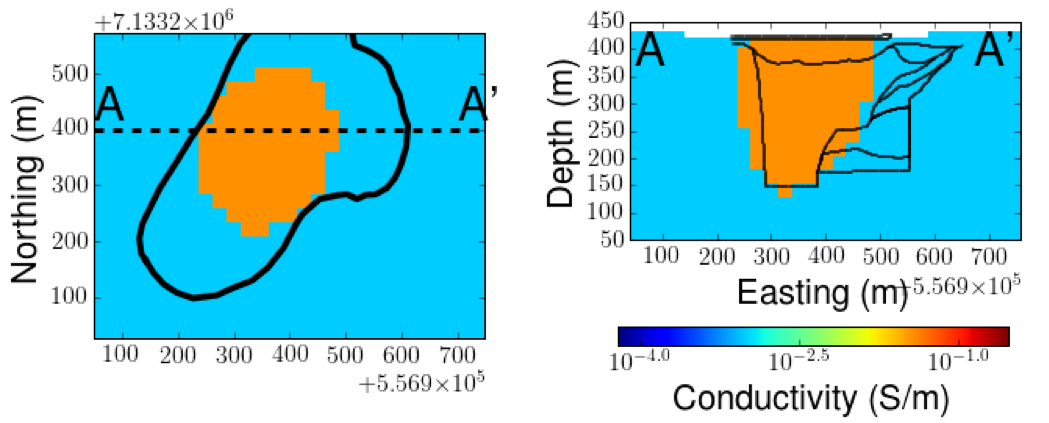
\includegraphics[width=0.8\textwidth]{figures/paramcond.png}
  \caption{Recovered conductivity model from parametric inversion of VTEM data near DO-27. Left and right panel shows plan and section views of the recovered conductivity model. Black solid line shows boundary of different kimberlites obtained from Fig. ~\ref{Fig:tkcgeo}(c). }
  \label{Fig:paramcond}
\end{figure}

\begin{figure}[htb]
  \centering
  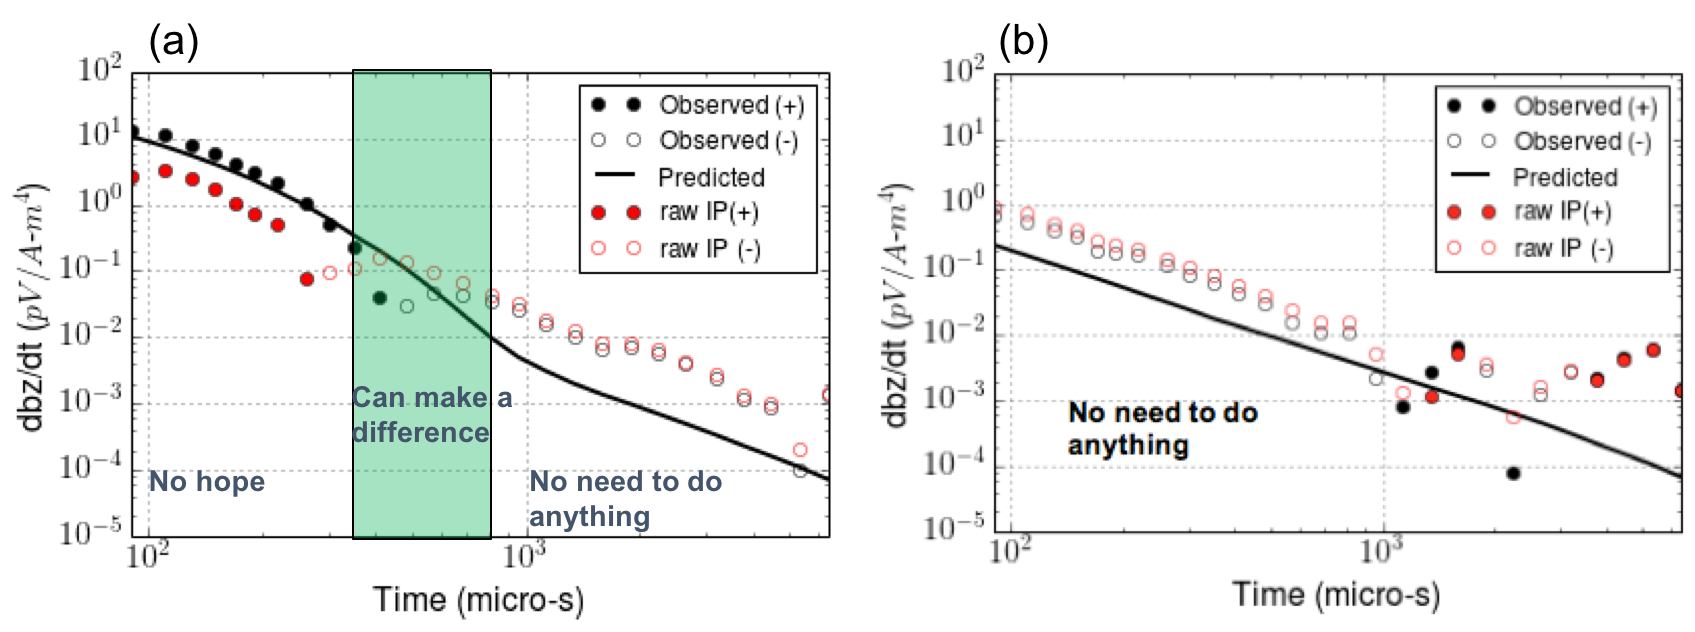
\includegraphics[width=0.8\textwidth]{figures/decoupledecay.png}
  \caption{Time decaying curves of observed, predicted and IP resposnes. Two stations near (a) DO-27) and (b) DO-18. Those are makred as black and white solid dots in Fig. ~\ref{Fig:decouplemap}, respectively.}
  \label{Fig:decoupledecay}
\end{figure}

\begin{figure}[htb]
  \centering
  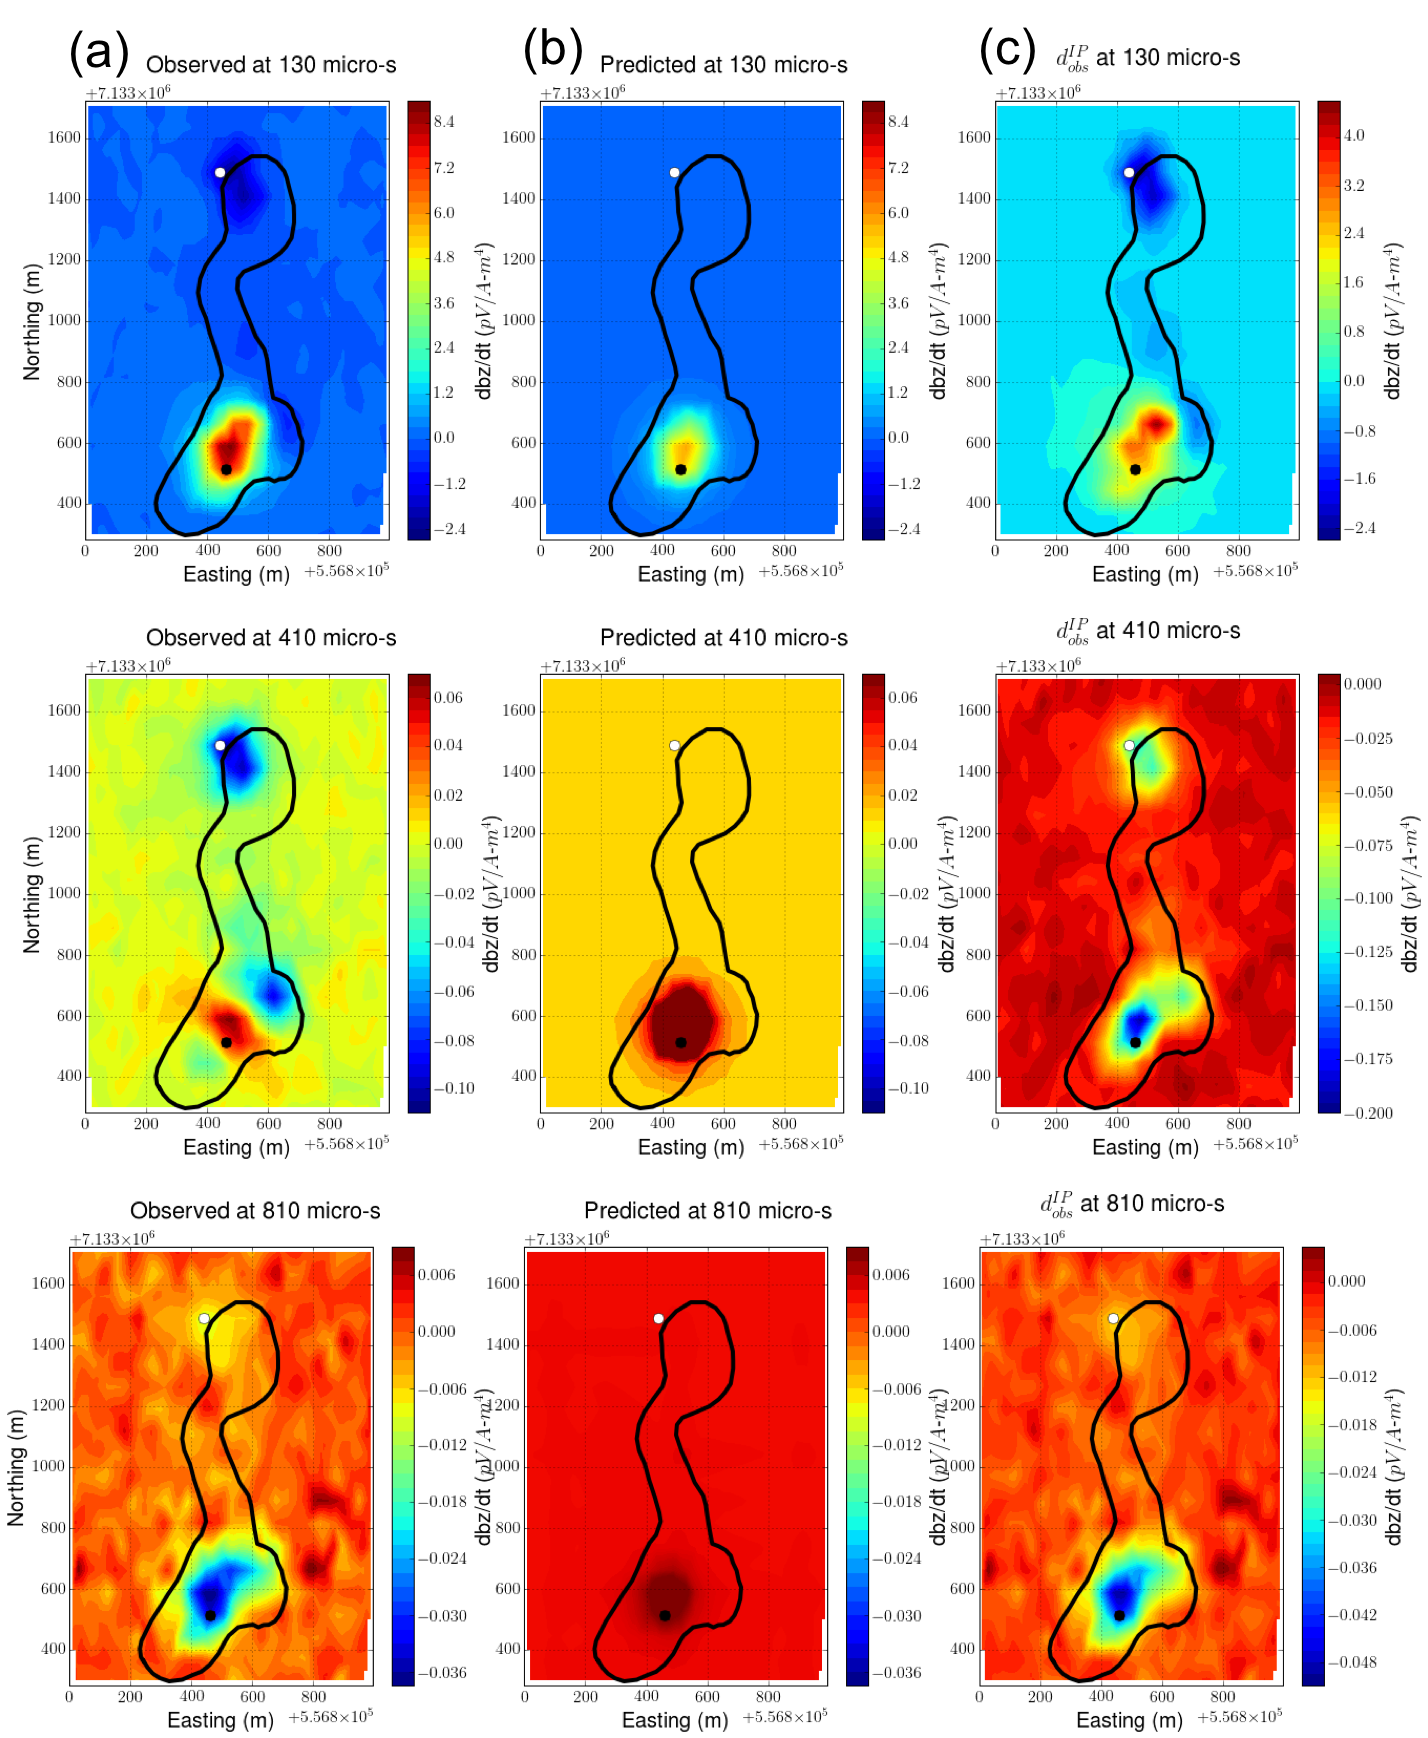
\includegraphics[width=0.8\textwidth]{figures/decouplemap.png}
  \caption{Maps of (a) observed, (b) predicted and (c) raw IP responses at TKC region. Top, middle, and bottom pannels correspondingly indicate times at 130, 410, and 810 micro-s. }
  \label{Fig:decouplemap}
\end{figure}

\subsection{3D IP inversion}
The second stage of the IP inversion procedure is recovering 3D pseudo-chargeability distribution by using linear sensitivity function shown in eq. ~\ref{eq:linearIPdatum}. Computing the sensitivity function is dependent upon the 3D conductivity model (See Sections \ref{appendix: linearization} for further details). This could be a problem for us because we only of localized conductivity model near DO-27 as shown in Fig. ~\ref{Fig:paramcond}. Fortunately, we have airborne frequency domain EM data acquired with a  Dighem system and these data do not show distinctive IP features like negative transients in ATEM data. By cooperatively inverting this data set with the parametric conductivity model we have recovered 3D conductivity model in the overall region of TKC as shown in Fig ~\ref{Fig:PetaSections} (a). Similar to the sensitivity function for DCIP \cite[]{doug1994}, the  sensitivity function shown in eq. ~\ref{eq:linearIPdatum} is not very dependent on conductivity \cite[]{Kang2015c}. Nonetheless, using the closest conductivity model to the true earth will provide us best inversion outputs. The conductivity model shown in Fig. ~\ref{Fig:PetaSections}(a) is our best estimate thus, we use this conductivity model to compute the sensitivity function. 

We apply our 3D IP inversion to the IP data and recover a 3D pseudo-chargeability at each time channel. Fig ~\ref{Fig:PetaSections}(b), (c) and (d) correspondingly show recovered pseudo-chargeability at 130, 410, and 810 micro-s. 
Four chargeable bodies (A1-A4) are imaged near DO-18 and -27. A1 shows the greatest pseudo-chargeability at 130 micro-s. Both A1 and A2 are seen at this time, but they almost disappear at 810 micro-s. The anomalies  A3 and A4 are recovered close to DO-27. A3 is close to the eastern boundary of kimberlite A3. The  chargeable body associated with A3 shows up at all three times. A4 is primarily  located near the western vertical boundary of DO-27 pipe. It is was not evident at 130 micro-s, was clearly visible at 410 micro-s, and has a strong response at 810 micro-s.  These different time decaying features of the  four chargeable bodies observed in the recovered pseudo-charegeability suggests that additional IP information may be extracted. As we illustrated in our IP inversion procedure (Fig. ~\ref{Fig:workflow}), as a final step we could interpret these recovered pseudo-chargeability to extract intrinsic IP information. As a first order approach, we performed cell-by-cell curve fitting approach, which fits pseudo-chargeability at each cell to extract Cole-Cole parameter assuming Debye model ($c$=1). Detailed description for this simple approach is shown in Section ~\ref{appendix: extract_intrinsicIP}. We only apply this cell-by-cell approach to regions where we have considerable pseudo-chargeability at arbitrary times. Fig. ~\ref{Fig:tauetamap} shows the recovered time constant and intrinsic chargeability near the four chargeable bodies. The recovered time constant for A1-A3 are $\sim$ 100 micro-s, while  that for A4 is $\sim$ 1000 micro-s. Chargeability of four bodies are mostly ranging from 0.1-0.4. Although not shown here, these results agreed well with IP measurements from core samples. Importantly, the recovered time constants show a possible distinction between DO-18 and DO-27 pipes. Considering DO-27 is more diamondiferous kimberlite pipe compared to DO-27, this may be an important observations. 

\begin{figure}[htb]
  \centering
  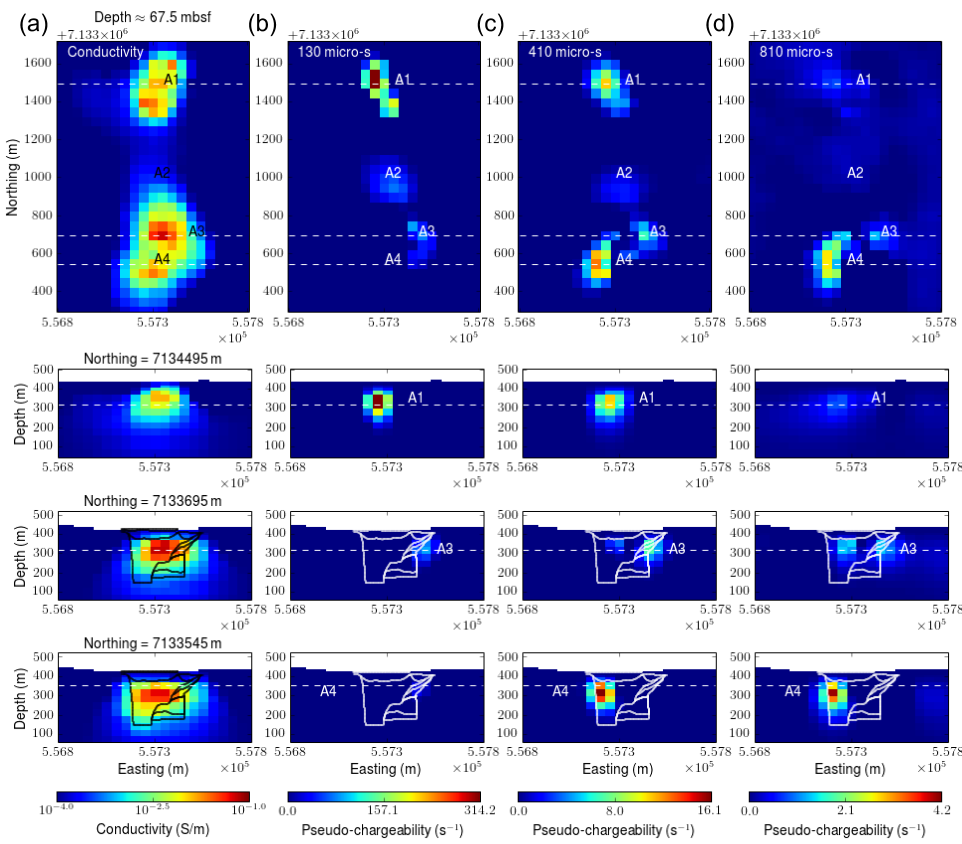
\includegraphics[width=0.8\textwidth]{figures/PetaSections.png}
  \caption{(a) Recovered 3D conductivity model. 3D pseudo-chargeability model at (a) 130, (b) 410, and (c) 810 micro-s. Top panel shows plan view map of models. Second b, third and last panels show easting section views in decreasing order in northing direction. }
  \label{Fig:PetaSections}
\end{figure}
\begin{figure}[htb]
  \centering
  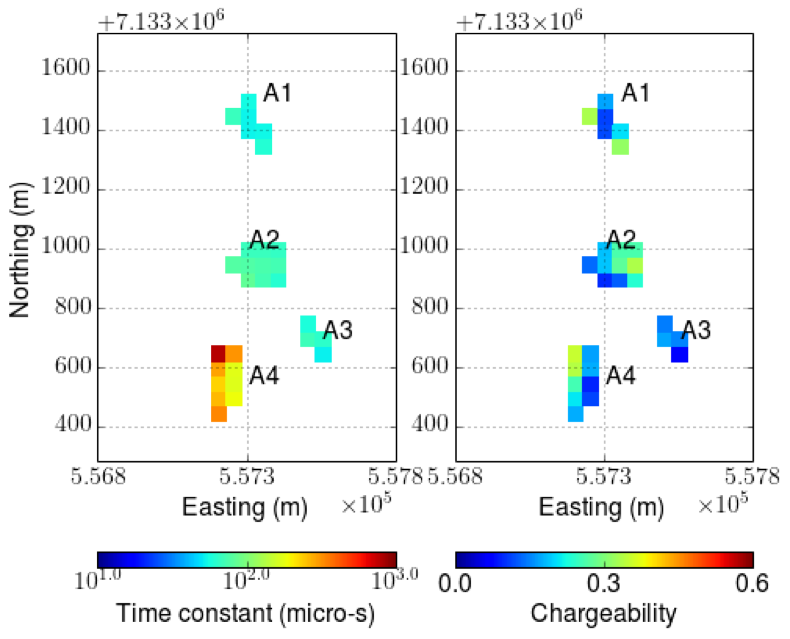
\includegraphics[width=0.6\textwidth]{figures/tauetamap.png}
  \caption{Recovered time constant (left panel) and chargeability (right panel) on plan view map. }
  \label{Fig:tauetamap}
\end{figure}
\clearpage

\section{CONCLUSIONS}
We have developed an IP inversion workflow to recover a 3D distribution of IP information from TEM data. The processing contains estimation of a background conductivity, removal of EM coupling, estimation of a possible residual field induced by incorrect conductivity distribution of the earth, and carrying out a 3D inversion to recover a pseudo-chargeability. To realize this workflow, mathematical foundations were constructed by decomposition of the observed EM fields and the linearization of IP responses as a function of pseudo-chargeability. Different excitation mechanism of inductive source from galvanic source was carefully considered to construct a linear form of IP response. Most challenging case for our methodology: ATEM (multiple sources with a single receiver) is successfully treated, and this will be the basement of our following researches. 

For the remainder of my Ph.D., the primary areas of research will be:
\begin{itemize}
  \item Applying our IP inversion procedure for galvanic source IP surveys
  \item Extracting intrinsic IP information such as Cole-Cole parameters
  \item Connecting recovered IP information to possible geological sources of IP
  \item Depth resolution of airborne IP
\end{itemize}

\subsection{Intellectual merits and impact}
In contrast to galvanic source IP, which is a mature technique in mining application, exploiting IP effects in inductive source system is still a young technique. Most of interpretations about inductive source IP (ISIP) are based on the assumption that the conductivity of the earth is  one-dimensional. We treated ISIP problem in 3D, and constructed linear functional which simulates ISIP responses, and tested the methodology. There are two important aspects that this linear functional provides:
\begin{itemize}
  \item Physical understanding of polarization charge build-up and its impact on the observed data
  \item Cost effective forward modelling which allows us to run a fast 3D IP inversion
\end{itemize}
In addition,  we suggested a comprehensive IP inversion procedure, which can be applied to both galvanic and inductive sources TEM data. We are planning to apply this procedure to different types of IP data including EIP, MIP, and ISIP. This will provide a comprehensive methodolgy  that one can use to obtain 3D distribution of IP information from TEM data.

\subsection{Research timeline}
\begin{enumerate}
  \item Linearization of time domain IP data and applying the IP inversion procedure
  \begin{itemize}
    \item Multiple inductive sources with a single receiver (\cite{Kang2015c}, submitted to $\mathit Geophysical \ Journal \ International$)
    \item Galvanic source (on-going)
    \item A single inductive source with multiple receivers 
  \end{itemize}
  \item Airbonre IP
  \begin{itemize}
    \item EM decoupling and 3D IP inversion (\cite{Kang2015a}, preparing a paper to submit $\mathit Geophysics$)
    \item Airborne IP for Kimberlite explorations (\cite{Kang2015b}, preparing a paper to submit $\mathit Geophysics \ Interpretation$)
    \item Depth resolution of airborne IP
  \end{itemize}  
\end{enumerate}
\subsection{Relevant conference presentations - (* = presenting author)}
\begin{itemize}
\item
$\mathbf{Kang, S.}$*, Oldenburg, D. W., (2014), On recovering induced polarization information from airborne time domain EM data, $SEG \ Extended \ Abstracts$ - Winner: Best student talk, Mining Section.
\item
$\mathbf{Kang, S.}$*, Oldenburg, D. W., (2015), Recovering IP information in airborne-time domain electromagnetic data, $ASEG \ Extended \ Abstracts$.
\item
$\mathbf{Kang, S.}$*, Oldenburg, D. W., (2015), 3D IP Inversion of Airborne EM data at Tli Kwi Cho, $ASEG \ Extended \ Abstracts$.
\item
$\mathbf{Kang, S.}$*, Rowan, C., Lindsey, H., and Oldenburg, D. W., (2015), Moving between dimensions in EM inversions, $SEG \ Extended \ Abstracts$.
\end{itemize}

\subsection{Peer reviewed publications}
\begin{itemize}
\item
Rowan, C., \&, $\mathbf{Kang, S.}$, \& Lindsey, H., Pidlisecky, A., and Oldenburg, D. W., (2015). SimPEG: An Open Source Framework for Simulation and Gradient Based Parameter Estimation in Geophysical Applications, $\mathit Computers \ and \ Geoscience$.
\item 
$\mathbf{Kang, S.}$, \& Oldenburg, D. W., (2015). On recovering distributed IP information from inductive source time domain electromagnetic data,  $\mathit Geophysical \ Journal \ International$ (submitted).
\end{itemize}

% \bibliographystyle{plain}
\bibliographystyle{/Users/sgkang/Projects/IPresearch/journals/atemIP_gji/gji}
\bibliography{../reference}

\clearpage
\section{APPENDICIES}
\label{section:appendix}
\subsection{Pseudo-chargeability}
\label{appendix: pseudochargeability}
Combining eq. (\ref{eq:sigmat}) and  $\j(t) = \sigma(t)\otimes \e(t)$ with $\j(t)=\j^F + \j^{IP}$ we obtain
\begin{linenomath*}
\begin{equation}
  \j^{IP} = \siginf \e^{IP} + \j^{pol}, 
  \label{eq:IP_current}
\end{equation}
\end{linenomath*}
where $\j^{pol} = \dsig(t)\otimes\e(t)$. 
From the previous section, we identified different characteristics of polarization charge builup for the inductive and galvanic sources. 
More specifically, we consider two cases: a) galvanic source without EM induction and b) inductive source with EM induction. The first case corresponds to EIP \cite[]{seigel1959}, and the second is ISIP.
A fundamental difference for these two cases were: 
\begin{itemize}
  \item EIP: the electric field is instantaneous due to the steady-state electric field (Fig. ~\ref{Fig:singlpixelE}(a))
  \item ISIP:  the electric field in the off-time is not zero, but increases to a peak and then decays as shown in Fig. ~\ref{Fig:singlpixelE} (b)
\end{itemize}

The polarization current for the two different sources will be significantly affected by these different electric fields as shown in Fig. ~\ref{Fig:singlpixelE}. 
To capture this difference in a linearized kernel for the IP response, we define pseudo-chargeability, $\peta(t)$ as 
\begin{linenomath*}
\begin{equation}
  \peta(t) = -\frac{\j^{pol}(t)}{\j^{\ ref}},
  \label{eq:pseudochargeability_0}
\end{equation}
\end{linenomath*}
where the reference current ($\j^{ref}$) is defined as 
\begin{linenomath*}
\begin{equation}
  \j^{\ ref} = \siginf \eref.
  \label{eq:reference_current}
\end{equation}
\end{linenomath*}
Here $\eref$ is the reference electric field and both $\j^{\ ref}$ and $\eref$ are static fields that are independent of time. 
The pseudo-chargeability defined in eq. (\ref{eq:pseudochargeability_0})  is the ratio of  the polarization current to the reference current. This is a small quantity and it plays an essential role in our linearization. 

To evaluate the pseudo-chargeability, we have to identify the reference current or reference electric fields. For the EIP case, the electric field, when there is no IP present, is independent of time as shown in Fig. ~\ref{F:DCEM_F_current}(a). For the inductive source however, the electric field does not achieve a steady-state, but increases to a  peak then decreases. 

Each pixel in the earth has its own reference electric field and time thus  both $\eref$ and $t^{\ ref}$ have a 3D distribution. 
For both EIP and ISIP cases, we mathematically present our choice of the reference electric field as
\begin{linenomath*}
\begin{equation}
  \eref = \e^{F}(t) \otimes \delta(t-t^{\ ref}). 
  \label{eq:reference_electricfield}
\end{equation}
\end{linenomath*}
The reference time for the EIP case can be any time in the on-time, because the fundamental electric field for the EIP case does not change in on-time. 

By rearranging eq. (\ref{eq:pseudochargeability_0}), we obtain 
\begin{linenomath*}
\begin{equation}
  \j^{pol} = -\jref\peta(t). 
  \label{eq:polarization_current_concept}
\end{equation}
\end{linenomath*}
This states that the polarization current has an opposite direction to the reference current, and is proportional to the pseudo-chargeability ($\peta(t)$). 
This conceptual model about the polarization current shown in eq. (\ref{eq:polarization_current_concept}) is consistent with \cite{seigel1959}'s result. We note, that for any pixel, even though  $\eref$  attains the same value for an ISIP survey as for an EIP survey, the pseudo-chargeability resulting from  an ISIP survey  will be less than that from an EIP survey. We can infer from this that  linearization techniques, which  have worked so well in EIP problems, should be successful in ISIP problems. 
\begin{figure}  
  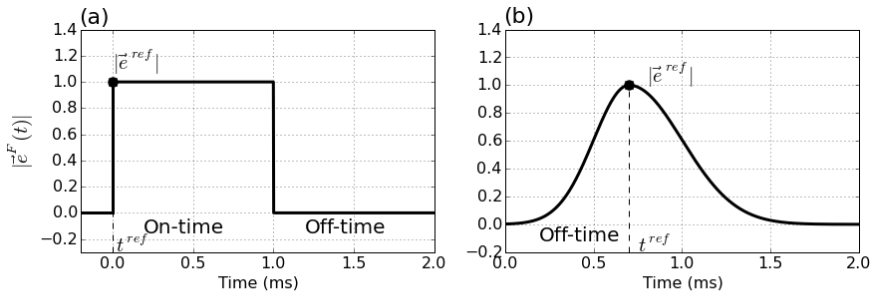
\includegraphics[width=1.0\textwidth]{figures/DCEM_F_current.png} 
  \caption{Conceptual diagram for the amplitude of the fundamental electric fields. (a) EIP and (b) ISIP cases.}
  \label{F:DCEM_F_current}
\end{figure}   

\subsection{Linearization}
\label{appendix: linearization}
Following from the methodologies in EIP, our goal is to express the IP response ($\dip$) as a function of the pseudo-chargeability $(\peta(t))$ in time  $\dip(t) = G[\peta(t)]$, where $G[\cdot]$ is a linear operator which is independent of time. In doing this we first consider a general EM system which is applicable to galvanic or inductive sources. 
For any pixel  volume in the earth the amplitude and direction of the  electric field can vary dramatically  in time and this results in a complicated  IP charging process. If substantial polarization currents are developed however, they will correspond to a maximum electric field or reference current aligned in a constant direction. Our formulation focuses on this aspect. We assume that the final large-scale IP response observed in the data is the result of  pixels being charged with an electric field in a specific direction but with a variable amplitude. Let $\e(t)$ be approximated as
\begin{linenomath*}
\begin{equation}
  \e(t) \approx \eref \hat{w}(t),
  \label{eq: e_with_eref}
\end{equation}
\end{linenomath*}
where $\hat{w}(t)$ is defined as:
\begin{linenomath*}
\begin{equation}
  \hat{w}(t) = P_0[w^{ref}(t)].
  \label{eq: we}
\end{equation}
\end{linenomath*}
Here a projection ($P_0[\cdot]$) of an arbitrary function, $f(t)$ is
\begin{linenomath*}
\begin{equation}
  P_0[f(t)] = \left\{ 
  \begin{array}{l l}
    f(t) & f(t) \ge 0 \\
    0 & \text{if } f(t) < 0, 
  \end{array}\right.
  \label{eq: P0}
\end{equation}
\end{linenomath*}
and
\begin{linenomath*}
\begin{equation}
  w^{ref}(t) = \frac{\e^F(t)\cdot\eref}{\eref\cdot\eref}.
  \label{eq: wref}
\end{equation}
\end{linenomath*}
Here $w^{ref}(t)$ is a dimensionless function that prescribes the time history of the electric field at each location along the direction of the chosen reference electric field ($\eref$).  Negative values of  $w^{ref}(t)$ are set to zero in accordance with our conceptual model that polarization currents have an opposite direction to the reference current (eq. \ref{eq:polarization_current_concept}).
We redefine the pseudo-chargeability as
\begin{linenomath*}
\begin{equation}
    \peta(t) = \peta^{I}(t)\otimes \hat{w}(t),
    \label{eq: pseudochargeability}
\end{equation}
\end{linenomath*}
where intrinsic pseudo-chargeability is 
\begin{equation}
  \peta^{I}(t) = -\frac{\dsig(t)}{\siginf}.
  \label{eq: intrinsic_peta}
\end{equation}
The polarization current, $\j^{pol}$ can be approximated with eq. (\ref{eq: intrinsic_peta}) as
\begin{linenomath*}
\begin{equation}
  \j^{pol}(t) \approx - \peta^{I}(t)\otimes \hat{w}(t)\jref.
\end{equation}
\end{linenomath*}
Substituting this into eq. (\ref{eq:IP_current}) yields
\begin{linenomath*}
\begin{equation}
  \j^{IP}(t) \approx \siginf\e^{IP}(t) - \peta^{I}(t)\otimes \hat{w}(t)\jref
\end{equation}
\end{linenomath*}
and this yields
\begin{linenomath*}
\begin{equation}
  \j^{IP}(t) \approx \siginf\e^{IP}(t) -\jref\peta(t).
  \label{eq: jip_EMIP}
\end{equation}
\end{linenomath*}

The second term, $-\jref\peta(t)$, correspond to polarization currents. The first term, $\siginf \e^{IP}(t)$ is usually omitted \cite[]{Smith1988a}. Here we include it and explore the conditions in which it is important. 
Because the reference current is static, any time-dependency in the polarization currents is encapsulated in the pseudo-chargeability. The buildup and decrease of polarization currents is a slow process and we assume therefore that this process does not produce induction effects ($\frac{\partial \b^{IP}}{\partial t} \approx 0$) and hence we can write 
\begin{linenomath*}
\begin{equation}
  \e^{IP} \approx  \e^{IP}_{approx} = -\grad\phi^{IP}.
  \label{eq: eip_approx}
\end{equation}
\end{linenomath*}

By taking the divergence of  eq. (\ref{eq: jip_EMIP}), substituting  $\e^{IP}$ with eq. (\ref{eq: eip_approx}), and carrying out some linear algebra, we obtain
\begin{linenomath*}
\begin{equation}
  \phi^{IP}(t) \approx -[\div \siginf\grad]^{-1}\div\jref\peta(t).
  \label{eq: phiIPapprox_general}
\end{equation}
\end{linenomath*}
By applying the gradient we obtain 
\begin{linenomath*}
\begin{equation}
    \e^{IP}_{approx} = \grad[\div \siginf\grad]^{-1}\div\jref\peta(t).
    \label{eq: eip_approx_full}
\end{equation}
\end{linenomath*}
Thus, the electric field due to the IP effect can be expressed as a function of $\peta(t)$ in time. 
This form is also applicable to the  EIP case.   

For an inductive source, the data is often either $\b$ or its time derivative and hence we also need to compute $\b^{IP}$ or its time derivative.
For this, we first compute $\j^{IP}$ then use the Biot-Savart law. 
By substituting eq. (\ref{eq: eip_approx_full}) into eq. (\ref{eq: jip_EMIP}), the approximated IP current density, $\j^{IP}_{approx}$ can be expressed as
\begin{linenomath*}
\begin{equation}
  \j^{IP}(t) \approx \j^{IP}_{approx} = \bar{S}\jref\peta(t),
  \label{eq: jip_approx}
\end{equation}
\end{linenomath*}
where
\begin{linenomath*}
\begin{equation}
  \bar{S} = \siginf\grad[\div \siginf\grad]^{-1}\div-\bar{I}
\end{equation}
\end{linenomath*}
and $\bar{I}$ is an identity tensor. 
Applying the Biot-Savart law we have:
\begin{linenomath*}
\begin{equation}
  \b^{IP}_{approx}(\vec{r}; t) = \frac{\mu_0}{4\pi}\int_{\Omega}  \frac{\bar{S}\j^{\ ref}(\vec{r}_s)\times\hat{r}}{|\vec{r}-\vec{r}_s|^2}\peta(t)d\vec{r}_s,
  \label{eq: BiotbIP_approx}
\end{equation}
\end{linenomath*}
where $\vec{r}_s$ indicates a vector for a source location, and $\hat{r}=\frac{\vec{r}-\vec{r}_s}{|\vec{r}-\vec{r}_s|}$.
If $\siginf\e^{IP}$ is omitted in  $\j^{IP}$ then the tensor, $\bar{S}$ becomes $-\bar{I}$. 
In this situation, the IP current is same as the polarization current, and it always has opposite direction to the reference current. 
This reversed current, along with Biot-Savart law,  provides a physical understanding about the negative transients in ATEM data when the earth is chargeable. 

Observed data are often the time derivative of $\b$, hence by taking time derivative to the eq. (\ref{eq: BiotbIP_approx}), we obtain
\begin{linenomath*}
\begin{equation}
  -\frac{\partial\b^{IP}_{approx}}{\partial t}(\vec{r}; t) = \frac{\mu_0}{4\pi} \int_{\Omega}  \frac{\bar{S}\jref(\vec{r}_s)\times\hat{r}}{|\vec{r}-\vec{r}_s|^2} \Big( -\frac{\partial \peta(t)}{\partial t} \Big) d\vec{r}_s.
  \label{eq: BiotbIPdt_approx}
\end{equation}
\end{linenomath*}
Here we have chosen to keep the minus signs in eq. (\ref{eq: BiotbIPdt_approx}) so that $-\frac{\partial \peta(t)}{\partial t}$ is positive when $\peta(t)$ is decaying in time. 
Accordingly, the IP datum is given by  $-\frac{\partial\b^{IP}}{\partial t}$. 

The IP fields shown in eqs (\ref{eq: eip_approx_full}), (\ref{eq: BiotbIP_approx}) and (\ref{eq: BiotbIPdt_approx}) are linear functionals of $\peta$ and the equations for a single time channel can be discretized in space as
\begin{linenomath*}
\begin{equation}
  \mathbf{d}^{IP} = \mathbf{G}\peta,
  \label{eq: dIP_lineareq}
\end{equation}
\end{linenomath*}
where $\mathbf{G}$ is the corresponding sensitivity matrix. 
In particular when the observed datum is the time derivative of $\b$, the linear relationship can be written as 
\begin{linenomath*}
\begin{equation}
  \mathbf{d}^{IP} = \mathbf{G}(-\frac{\partial \peta}{\partial t}\Big|).
  \label{eq: dIP_lineareq_dbdt}
\end{equation}
\end{linenomath*}
The representation in eq. (\ref{eq: dIP_lineareq}) is valid for galvanic and inductive sources but the two assumptions: a) $\e \approx \eref \hat{w}(t)$ and b) $\e^{IP} \approx -\grad\phi^{IP}$ need to be tested numerically for the case of inductive sources. 

%%% ===========================================================================
%%% SUBSECTION
\subsection{Handling multiple transmitters in ATEM surveys}
\label{subsection: Handling multiple transmitters in ATEM surveys}
The work for inductive sources in the previous sections has been developed for a single transmitter and 3D information about chargeability can be obtained if there are multiple receivers. For ATEM data however, we have only a single receiver location for each transmitter but we have multiple transmitter locations. 
Our goal is to alter the problem to work with an effective pseudo-chargeability. 

In our linearized eq. (\ref{eq: dIP_lineareq}), each transmitter has its own sensitivity and pseudo-chargeabilty. For our airborne case the sensitivity for the $k$-th transmitter is the $k$-th row of $\mathbf{J}$ and the pseudo-chargeability is $\peta^k$. The corresponding  IP datum is 
\begin{linenomath*}
\begin{equation}
  \dip_k(t) = \sum_{i=1}^{nC}J_{k,i}\peta^k_i (t), \ \ k=1, \ldots, nTx,
  \label{eq: dip_kthTx}
\end{equation}
\end{linenomath*}
where $nTx$ is the number of transmitters, $nC$ is the number of cells in the domain, and $J_{k,i}$ indicates an element of the Jacobian matrix for the $k$-th transmitter and the $i$-th cell. We want to replace $\peta^k_i$ with a single effective pseudo-chargeabilty $\peta^k$ and therefore write the IP datum as 
\begin{linenomath*}
\begin{equation}
  \dip_k(t) = \sum_{i=1}^{nC}J_{k,i}\peta_i (t), \ \ k=1, \ldots, nTx,
  \label{eq: dipeff_kthTx}
\end{equation}
\end{linenomath*}
The waveforms are different for each transmitter and hence this representation cannot be exact. To examine the implications of this it suffices to look at the contribution of any volumetric pixel. Each pixel contributes to all of the IP data but in differing amounts. The total contribution of the  $i$-th pixel to the $nTx$ data set at a single time is  
\begin{linenomath*}
\begin{equation}
  q_i =\sum_{k=1}^{nTx} J_{k,i} \peta^k_i(t), \ \ i=1, \ldots, nC.
  \label{eq: dip_hat}
\end{equation}
\end{linenomath*}
Our goal is to find an effective chargeability that produces the same net effect on the measured data. We search for a transmitter-independent $\peta_i$ such that 
\begin{linenomath*}
\begin{equation}
  q_i^{est} =\sum_{k=1}^{nTx} J_{k,i} \peta_i(t), \ \ i=1, \ldots, nC.
  \label{eq: dip_tilde}
\end{equation}
\end{linenomath*}
Minimizing the least squares difference between eqs (\ref{eq: dip_hat}) and (\ref{eq: dip_tilde}) yields
\begin{linenomath*}
\begin{equation}
  \peta_i(t) = \frac {\Sigma_{k=1}^{nTx} J_{k,i}^2\peta^k_i(t)} {\Sigma_{k=1}^{nTx} J_{k,i}^2} = \sum_{k=1}^{nTx} a^k_i \peta^k_i(t), \ \ i=1, \ldots, nC.
  \label{eq: petaeff}
\end{equation}
\end{linenomath*}
where normalized weight ($a^k_i$) is 
\begin{linenomath*}
\begin{equation}
  a^k_i = \frac {J^2_{k,i}} {\Sigma_{k=1}^{nTx} J^2_{k,i}}, \ \ i=1, \ldots, nC.
  \label{eq: normalized_weights}
\end{equation}
\end{linenomath*}

With the above understanding about how $\peta_i$ relates to the $\peta_i^k$ from each transmitter we can proceed  as follows. Firstly, from eq. (\ref{eq: pseudochargeability}) we have 
\begin{linenomath*}
\begin{equation}
  \peta_i^k(t) =\peta^I \otimes \hat{w}^{k}_i(t) 
  \label{eq: peta_transmitters}
\end{equation}
\end{linenomath*}
Substituting eqs (\ref{eq: peta_transmitters}) into (\ref{eq: petaeff}) allows us to write
\begin{linenomath*}
\begin{equation}
  \peta_i(t) = \peta^I(t) \otimes w^e_i(t),
\end{equation}
\end{linenomath*}
where we define effective time history of the electric field, $w^e_i(t)$ as 
\begin{linenomath*}
\begin{equation}
  w^e_i(t)= \sum_{k=1}^{nTx} a^k_i \hat{w}^{k}_i(t), \ \ i=1, \ldots, nC.
  \label{eq: we_eff}
\end{equation}
\end{linenomath*}

The above equations shows that the pseudo-chargeabilty for any pixel recovered from the inversion is equal to the convolution of the intrinsic pseudo-chargeability ($\peta^I(t)$) with an effective time history of the electric field ($w^e(t)$). Although it is somewhat involved, the $w^e(t)$ associated with each pixel can be evaluated by knowing the electric fields associated with the fundamental EM problem. Ultimately this allows us to estimate the parameters associated with the intrinsic pseudo-chargeability in the same manner as outlined for the case with a single transmitter. 

%%% ===========================================================================
%%% SUBSECTION
\subsection{3D IP inversion with a linearized kernel}
\label{appendix: 3DIPinversion}
The linear inverse problem to recover chargeability is straightforward and is described in \cite{doug1994}. 
We rewrite eq. (\ref{eq: dIP_lineareq}) as
\begin{linenomath*}
\begin{equation}
  \mathbf{d}^{pred} = \mathbf{G}\mathbf{m},
  \label{eq9}
\end{equation}
\end{linenomath*}
where $\mathbf{G}$ is the  sensitivity matrix of linear problem, which corresponds to $\mathbf{G}$ shown in eq. (\ref{eq: dIP_lineareq}). 
Here, $\mathbf{d}^{pred}$ represents IP responses at a single time channel, $\mathbf{m}$ denotes model parameters, which can be either $\peta$ or $-\frac{\partial \peta}{\partial t}\big|$ at the same time. 
In our work here we invert each time channel of $d^{IP}$, separately. 

The solution to the inverse problem is the model $\mathbf{m}$ that solves the optimization problem
\begin{linenomath*}
\begin{equation}
  minimize \ \phi =  \phi_d(\mathbf{m}) + \beta\phi_m(\mathbf{m}) \\
  s.t. \ 0 \le \mathbf{m},
  \label{eq10}
\end{equation}
\end{linenomath*}
where $\phi_d$ is a measure of data misfit, $\phi_m$ is a user-defined model objective function and $\beta$ is regularization or trade-off parameter. We solve this optimization problem using a projected Gauss-Newton method \cite[]{Kelley}. 
The value of $\beta$ is determined using a cooling technique where $\beta$ is progressively reduced from some high value. The inversion is stopped when the tolerance is reached (cf. \cite{DougTutorial, Kang2014}). 

We use the sum of the squares to measure data misfit
\begin{linenomath*}
\begin{equation}
  \phi_d = \| \mathbf{W_d}(\mathbf{G}\mathbf{m}-d^{obs}|)\|^2_2 =
  \sum^N_{j=1}(\frac{\mathbf{d}^{pred}_j-\mathbf{d}^{obs}_j}{\epsilon_j}),
  \label{eq11}
\end{equation}
\end{linenomath*}
where $N$ is the number of the observed data and $\mathbf{W_d}$ is a diagonal data weighting matrix which contains the reciprocal of the estimated uncertainty of each datum ($\epsilon_j$) on the main diagonal,  $\mathbf{d}^{obs}$ is a vector containing the observed data, $\mathbf{d}^{pred}$ is a vector containing calculated data from a linear eq. given in eq. (\ref{eq9}).
The model objective function, $\phi_m$, is a measure of the amount structure in the model and upon minimization this will generate a smooth model which is close to a reference model, $m_{ref}$. 
We define $\phi_m$ as
\begin{linenomath*}
\begin{equation}
  \phi_m = \sum_{i=s,x,y,z} \alpha_i\| \mathbf{W}_i\mathbf{W}(\mathbf{m}-\mathbf{m}_{ref})\|^2_2,
  \label{eq12}
\end{equation}
\end{linenomath*}
where $\mathbf{W}_s$ is a diagonal matrix, and $\mathbf{W}_x$, $\mathbf{W}_y$ and $\mathbf{W}_z$ are discrete approximations of the first derivative operator in $x$, $y$ and $z$ directions, respectively.  
The $\alpha$'s are weighting parameters that balance the relative importance of producing small or smooth models, and $\mathbf{W}$ stands for model weighting matrix \cite[]{LiMag3D}.

%% ===========================================================================
%% SUBSECTION
\subsection{Extracting intrinsic IP parameters}
\label{appendix: extract_intrinsicIP}
The output of our IP inversion is a 3D distribution of the pseudo-chargeability at multiple time channels. 
As its name suggests, pseudo-chargeability is not an intrinsic IP parameter like chargeability, but it is a convoluted property between $\peta^{I}(t)$ and $\hat{w}(t)$:
\begin{linenomath*}
\begin{equation}
  \peta(t) = \peta^{I}(t) \otimes \hat{w}(t),
  \label{eq: pseudochargeability_petaI}
\end{equation}
\end{linenomath*}
with the definition of intrinsic pseudo-chargeability (eq. \ref{eq: intrinsic_peta}).
We would now like to use the $\peta(t)$ as the “data” and recover intrinsic parameters such as $\eta, \tau, c$ in a Cole-Cole model. Assuming a Debye model ($c$=1), we obtain
\begin{linenomath*}
\begin{equation}
    \peta^{I}(t) = \frac{\eta}{(1-\eta)\tau}e^{-\frac{t}{(1-\eta)\tau}},
    \label{eq: intrinsic_peta_debye}
\end{equation}
\end{linenomath*}
Since we have $\siginf$ we can compute $\hat{w}(t)$, which is the time history of the electric field. 
Accordingly, we can unravel the recovered pseudo-chargeability to extract intrinsic IP parameters such as chargeability($\eta$) and time constant ($\tau$). 
We use a gradient-based optimization and thus we need the sensitivity function for the pseudo-chargeability (eq. \ref{eq: pseudochargeability_petaI}) with respect to $\eta$ and $\tau$. 
To simplify this procedure, we rewrite intrinsic pseudo-chargeability as 
\begin{linenomath*}
\begin{equation}
  \peta^{I}(t) = a e^{-bt},
\end{equation}
\end{linenomath*}
where $a = \frac{\eta}{(1-\eta)\tau}$ and $b = \frac{1}{(1-\eta)\tau}$. 
Then we take derivative of $\peta(t)$ with regard to $a$ and $b$:
\begin{linenomath*}
\begin{equation}
  \frac{\partial \peta(t)}{\partial a} = e^{-bt} \otimes \hat{w}(t),
\end{equation}
\end{linenomath*}
\begin{linenomath*}
\begin{equation}
  \frac{\partial \peta(t)}{\partial b} = -ate^{-bt} \otimes \hat{w}(t).
\end{equation}
\end{linenomath*}
With these sensitivity functions, we can set up an inverse problem, and recover $a$ and $b$. 
Chargeability and time constant can be obtained by using $a$ and $b$:
\begin{linenomath*}
\begin{equation}
  \eta =  \frac{a}{b},
\end{equation}
\end{linenomath*}
\begin{linenomath*}
\begin{equation}
  \tau =  \frac{1}{(1-a/b)b}.
\end{equation}
\end{linenomath*}
We apply this inversion separately to each cell in the recovered pseudo-chargeability  in a manner similar to \cite[]{Yuval1997}.
For the better representation of time-dependent conductivity, a different parameterization such as stretched-exponential \cite[]{Kohlrausch1854} or Cole-Cole model with variable $c$ can be implemented. 
\end{document}

